\documentclass[MathsNotesBase.tex]{subfiles}



\date{\vspace{-6ex}}


\begin{document}

\searchableChapter{Algebra}{abstract algebra, complex numbers}

	\searchableSection{Group Theory}{abstract algebra}
	
	\searchableSubsection{Groups}{abstract algebra}{\bigskip
		
		\boxeddefinition{
		A binary operation is a function,
		\[ f:G \times G \longmapsto G \]
		which - by the definition of a function - maps a unique tuple from $G \times G$ to a unique value in the codomain $G$.
		}
		\bigskip
		
		\boxeddefinition{
		Let $G$ be a set and $*$ a binary operation on $G$ and denote this ($G,*$). Then ($G,*$) is a \textbf{group} if:
		\paragraph*{closure} $\forall x,y \in G, x * y \in G$;
		\paragraph*{associativity} $\forall x,y,z \in G, (x * y) * z = x * (y * z)$;
		\paragraph*{identity} $\exists e \in G \suchthat \forall x \in G, e*x = x*e = x$;
		\paragraph*{inverse} $\forall x \in G, \exists x^{-1} \in G \suchthat x * x^{-1} = x^{-1} * x = e$.\\\\
		These are known as the \textbf{group axioms}.
		}
		
		
		
		\bigskip\smallskip
		\boxeddefinition{
		The group is an \textbf{Abelian group} if it has the additional property:	
		\paragraph*{commutativity} $\forall x,y \in G, x * y = y * x \in G$.
		}
		
		\bigskip\smallskip 
		\notation{from here on we will use juxtaposition notation for the group operation (so $xy = x * y$) and (usually) $1$ for the identity element instead of $e$. This is known as \textit{multiplicative notation}.}
		
		\labeledTheorem{Suppose an associative law of composition is given on a set $S$. Then there is a unique way to define a product of $n$ elements ${ a_1, \dots, a_n }$ for any ${ n \in \N{} }$.}{associative_law_gives_unique_n-ary_products}
		\begin{proof}
			Denote the product of $n$ elements as ${ [a_1 \dots a_n] }$. We show that a product can be defined with the following properties:
			\begin{enumerate}[label=(\roman*)]
				\item{${ [a_1] = a_1 }$;}
				\item{${ [a_1a_2] = a_1 * a_2 }$ is defined by the law of composition;}
				\item{for any integer $i$ such that ${ 1 \leq i \leq n }$, ${ [a_1\dots a_n] = [a_1\dots a_i][a_{i+1}\dots a_n] }$.}
			\end{enumerate}
			Following a proof by induction, firstly note that the product is defined for ${ n \leq 2 }$ by (i) and (ii) and that (ii) also satisfies the requirement (iii). Then, assume that the product is defined for ${ n \leq 2 }$ and that this product is the unique product satisfying (iii).\\
			Then the induction step is to show that,
			\[ [a_1\dots a_n] = [a_1\dots a_{n-1}][a_n] \]
			\TODO{complete this from Artin[56]}
		\end{proof}
		
		\bigskip\bigskip
		\subsubsection{Corollaries of the group axioms}
		The group operation is defined to map a unique tuple in $G \times G$ to a unique value in $G$ so that if we have $x,y \in G$ then $f((x, y)) = f(x,y) = xy \in G$ and for $a,b,c \in G$,
		\[ a = b \iff (c, a) = (c, b) \implies f((c, a)) = f((c, b)) \iff ca = cb \]
		\[ \therefore a = b \implies ca = cb \]
		
		Then, using all the group axioms - associativity, inverse and identity,
		\[ ca = cb \implies \inv{c}(ca) = \inv{c}(cb) \iff (\inv{c}c)a = (\inv{c}c)b \iff 1a = 1b \iff a = b \]
		
		Therefore we have the principle of cancellation,
		\[ ca = cb \implies a = b \]
		\textit{Note} that, since we have used the axioms of inverse and identity and the definitions of these require these elements to exhibit these properties from both the left and the right, the principle of cancellation can also be shown from both the left and the right. So, also,
		\[ ac = bc \implies a = b \]
		
		\bigskip\bigskip
		There are (at least) two approaches to finding the other consequences of the group axioms.
		\paragraph*{First approach.} We begin by noticing that the law of cancellation implies that,
		\subparagraph*{unique identity and inverses}$\forall a,x,b \in G, ax = b$ has a unique solution because,
		\[ ax = ax' \iff x = x' \]
		That unique solution is $a^{-1}b$. If $b=a$ we have $ax=a$ and $x$, by identity axiom, is an identity element. Since, the solution to this equation - $x$ - is unique, it follows that there is a unique value that is the identity element. Then, if we let $b$ be this unique identity element we have $ax=1$ and the unique solution, $x$, is the inverse of a, i.e. $\inv{a}$. Therefore, the inverses of group elements are also unique.
		
		\paragraph*{Second approach.} This approach begins by showing the uniqueness of the identity element solely using the defintion of the identity. Here, for clarity, we revert to using $e$ to denote the identity element.
		\subparagraph*{unique identity} Assume there are two identity elements, $e, e'$. Then, by the definition of the identity $ee' = e'e = e = e'$ so that there is a single value that has the property of the identity element.\\\\
		Then, using the definition of the inverse we have,
		\subparagraph{unique inverses} Assume there are two distinct inverses of an element $a$: $\inv{a}$ and $a'$. Then, 
		\begin{align*}
		&& a\inv{a} = 1 &= aa' &\sidecomment{defn. of inverse, uniqueness of identity}\\
		& \iff & \inv{a} &= a' &\sidecomment{law of cancellation}
		\end{align*}
		\bigskip\bigskip

		\paragraph*{Some Examples of Groups}
		\begin{itemize}
		\item{ ($\R{} \setminus \{0\}, \times)$ } is a group whereas ($\R{}, \times)$ is not a group because $0$ has no multiplicative inverse.
		\item{ ($\R{}, +)$ } is a group.
		\item{ The set of $n \times n$ invertible matrices is called the General Linear group and denoted $GL_n$  }
		\item{Let $G$ denote the set of matrices
			\[ G = \left\{
				\begin{pmatrix}
					a & b \\
					0 & 1
				\end{pmatrix}
			\; \middle\vert \; a,b \in \Z{}_7, \; a \neq 0 \right\}. \]
			Then $G$ is a group with respect to matrix multiplication (where all additions and multiplications are carried out in $\Z{}_7$). This is because closure can be shown by,
			\[
				\begin{pmatrix}
				a & b \\
				0 & 1
				\end{pmatrix}
				\begin{pmatrix}
				a' & b' \\
				0 & 1
				\end{pmatrix}
				=
				\begin{pmatrix}
				aa' & ab' + b \\
				0 & 1
				\end{pmatrix} \in G
			\]
			where the result is in $G$ because ${ aa' \neq 0 }$. Next we need to show that we have inverses. So we need to show existence in $G$ of matrices such that,
			\[
				\begin{pmatrix}
				a & b \\
				0 & 1
				\end{pmatrix}
				\begin{pmatrix}
				a' & b' \\
				0 & 1
				\end{pmatrix}
				=
				\begin{pmatrix}
				1 & 0 \\
				0 & 1
				\end{pmatrix} 
				\iff
				\begin{pmatrix}
				aa' & ab' + b \\
				0 & 1
				\end{pmatrix}
				=
				\begin{pmatrix}
				1 & 0 \\
				0 & 1
				\end{pmatrix}
			\]
			which implies that ${ aa' = 1 }$ and ${ ab' + b = 0 }$. Because we are in $\Z{}_7$ every non-zero element has a multiplicative inverse so we have,
			\[ a' = \inv{a} \eqand b' = -\inv{a}b \]
			so that,
			\[
				\inv{\begin{pmatrix}
				a & b \\
				0 & 1
				\end{pmatrix}}
				=
				\begin{pmatrix}
				\inv{a} & -\inv{a}b \\
				0 & 1
				\end{pmatrix}.
			\]
		}
		\end{itemize}
		
		\bigskip
		\subsubsection{Permutations and Symmetric Groups}\bigskip
		\boxeddefinition{A \textbf{permutation} is a bijection from a set to itself. Since permutations are bijective, they are invertible and since they are functions, function composition defines an associative law of composition over them. As a result, they form a group. 
		}
		\boxeddefinition{The \textbf{symmetric group} defined over a set is the group whose elements are the permutations of the objects of the set and whose law of composition is the composition of functions. The name probably comes from the study of symmetries of geometric objects that were eventually realised to be equivalent to permutations of the vertices.
		}
		\label{def:generating_set_of_group} 
		\boxeddefinition{A \textbf{generating set of a group} is a subset such that every element of the group can be expressed as a combination (under the group operation) of finitely many elements of the subset and their inverses.}
		
		\smallskip
		\notation{The symmetric group over the integers from 1 to n is denoted $S_n$. The symmetric group over a set $G$ may be denoted ${ Sym(G) }$.}\\
		
		\subparagraph{$\bm{S_2}$}
		The symmetric group $S_2$ consists of the two elements $i$ and $\tau$ which are, respectively, the identity map and the transposition which interchanges 1 and 2. The group composition law is described by the fact that the identity map is the identity of the composition and by the relation $\tau\tau = \tau^2 = i$. Which results in the multiplication table:	
		\[
		\begin{aligned}
			i &\cdot i &&= i \\
			i &\cdot \tau &&= \tau \\		
			\tau &\cdot i &&= \tau \\
			\tau &\cdot \tau &&= i \\
		\end{aligned}
		\]
		Note that the law of composition is commutative.
		\subparagraph{$\bm{S_3}$}\label{S_3}
		The symmetric group $S_3$ contains $3!$ elements. It is the smallest group whose law of composition is not commutative. It can be described using any two permutations of $\{1, 2, 3\}$. For example, if we take,
		\begin{align*}
			x =
			\begin{bmatrix}
			0 & 1 & 0 \\
			0 & 0 & 1 \\
			1 & 0 & 0 \\
			\end{bmatrix},\;
			y =
			\begin{bmatrix}
			0 & 1 & 0 \\
			1 & 0 & 0 \\
			0 & 0 & 1 \\
			\end{bmatrix}
		\end{align*}
		Then the permutations are,
		\[ \{1, x, x^2, y, xy, x^2y\} = \setc{x^iy^j}{0 \leq i \leq 2,\; 0 \leq j \leq 1} \]
		These are the elements of the group. The composition law over these elements is the function composition of these permutation functions and its multiplication table is characterized by the rules:
		\begin{align*}
			x^3 = 1,\; y^2 = 1,\; yx = x^2y
		\end{align*}
		These are derived directly from the permutations themselves. Note that this composition law is not associative as $yx \neq xy$. \\
		Any product of the elements $x,y$ and of their inverses can be brought into the form $x^iy^j$ with $i,j$ taking the ranges given above by repeated application of the above rules. To do so, we move all occurrences of $y$  to the right side using the last relation and bring the exponents into the indicated ranges using the first two relations:
		\begin{align*} 
			\inv{x}y^3x^2y &= x^2yx^2y = x^2(yx)xy = x^2(x^2y)xy = x^4(yx)y\\
						&= x^4(x^2y)y = x^6y^2 = (x^3)^2y^2 = 1 \cdot 1 = 1
		\end{align*}
		Rules like these that determine a complete multiplication table are called \textit{defining relations} for the group.	
	}
	
	
	\pagebreak
	\searchableSubsection{Subgroups}{abstract algebra}{\bigskip
		\boxeddefinition{
			A subset $H$ of a group $G$ is called a \textbf{subgroup} if it has the following properties:
			\begin{itemize}
				\item{\textbf{Closure:}} If $a \in H$ and $b \in H$ then $ab \in H$.
				\item{\textbf{Identity:}} $1 \in H$.
				\item{\textbf{Inverses:}} If $a \in H$ then $\inv{a} \in H$.
			\end{itemize}
			\note{These conditions show that the subset $H$ is a group with respect to the \textit{induced law of composition} created by applying the law of composition of $G$ on the members of $H$. Note that the associative property is not mentioned because the associativity of the composition of members of $G$ automatically carries over to $H$.}
		}
		
		
		\notation{If $H$ and $G$ are groups then we may write ${ H \leq G }$ to indicate that $H$ is a subgroup of $G$.}\\\\
		
		\note{Note that an alternative, more compact, formulation of the definition of a subgroup is as follows.\\\\
			\textbf{Let $\bm{G}$ be a group and ${\bm{ \emptyset \neq H \subseteq G }}$. Then $\bm{H}$ is a subgroup if}
			\[ \bm{ x,y \in H \implies \inv{x}y \in H }. \]
			This is because,
			\[ [(x,y \in H \implies xy \in H) \wedge (x \in H \implies \inv{x} \in H)] \iff (x,y \in H \implies \inv{x}y \in H). \]
			The implication,
			\[ [(x,y \in H \implies xy \in H) \wedge (x \in H \implies \inv{x} \in H)] \implies (x,y \in H \implies \inv{x}y \in H) \]
			is obvious. In the other direction,
			\[ (x,y \in H \implies \inv{x}y \in H) \implies [(x,y \in H \implies xy \in H) \wedge (x \in H \implies \inv{x} \in H)] \]
			is because, if we set ${ x = y }$,
			\[ \inv{x}x = e \in H \implies \inv{x}e = \inv{x} \in H \]
			and then, for ${ x \neq y }$,
			\[ \inv{x},y \in H \implies xy \in H. \]
		}
		

		Every group, at a minimum, has two trivial subgroups: the maximal subgroup - the group itself; and the minimal subgroup - the set containing just the identity. A subgroup that is neither of these is known as a \mbox{\textit{proper subgroup}}.\\
		
		\labeledProposition{Suppose $ H $ and $ K $ are subgroups of $ G $ such that neither ${ H \subseteq K }$ nor ${ K \subseteq H }$. Then ${ H \cup K }$ is not a subgroup of $ G $.}{union_of_subgroups_is_not_subgroup}
		\note{Note that it might be possible, for this proof, to just show that we have no reason to think that ${ H \cup K }$ is a subgroup (i.e. the definitions don't require it) so, in general, it is not. But, actually, we can show something much stronger: that ${ H \cup K }$ \textbf{cannot} be a subgroup. If we can easily show something stronger then in most cases it's going to add clarity.}
		\begin{proof}
			Since neither ${ H \subseteq K }$ nor ${ K \subseteq H }$ we can conclude that ${ H \setminus K }$ and ${ K \setminus H }$ are both non-empty. So, select an element from each, \[ h \in H \setminus K,\; k \in  K \setminus H. \]
			Then we have ${ h,k \in H \cup K }$ and if ${ H \cup K }$ were a group then the closure property of the group would require that \[ hk \in H \cup K.\] Assume ${ hk \in H \cup K }$. Then, ${ hk \in H }$ or ${ hk \in K }$. If ${ hk \in H }$ then the group properties of $H$ require that \[ \inv{h}hk = k \in H \] which contradicts the selection of $k$. We have a similar situation if ${ hk \in K }$. Therefore, ${ hk \not\in H \cup K }$.
		\end{proof}

		\bigskip
		\subsubsection{Additive Groups of Integers}
		Important examples are the subgroups of the additive group of integers $\Z{+}$. Denote the subset of $\Z{+}$ consisting of all multiples of a given integer $b$ by $b\Z{}$ such that,
		\[ b\Z{} = \setc{n \in \Z{}}{n = bk,\; k \in \Z{}} \]
		\labeledProposition{For any integer $b$, the subset $b\Z{}$ is a subgroup of $\Z{+}$ and every subgroup of $\Z{+}$ is of the form $b\Z{}$ for some integer $b$.}{bZ_subgroup}
		\begin{proof}
			$b\Z{}$ is a subgroup of $\Z{+}$ because,
			\begin{itemize}
				\item{$b(0) = 0 \in b\Z{}$;}
				\item{If $a_1,a_2 \in b\Z{}$ then $a_1 = bk_1, a_2 = bk_2$ for $k_1, k_2 \in \Z{}$ and so $a_1 + a_2 = bk_1 + bk_2 = b(k_1 + k_2) \in b\Z{}$}
				\item{For any $a = bk \in b\Z{}$, $-a = b(-k) \in b\Z{}$}
			\end{itemize}
			Now we need to prove that any subgroup of $\Z{+}$ is $b\Z{}$ for some $b$. Let $H$ be an arbitrary subgroup of $\Z{+}$. Then by subgroup properties,
			\begin{itemize}
				\item{$0 \in H$;}
				\item{If $a_1,a_2 \in H$ then $a_1 + a_2 \in H$}
				\item{For any $a \in H$, $-a \in H$}
			\end{itemize}
			We proceed to show that there is always some integer $b$ such that $H = b\Z{}$.\\
			Firstly, if $H$ is the minimal subgroup \{0\} then $H$ trivially conforms to $b\Z{}$ with $b = 0$.\\
			Otherwise, $\exists a \in H \suchthat a \neq 0$ then also $\exists -a \in H \suchthat -a \neq 0$. One of these must be a positive non-zero integer so there is at least one such member of $H$. We take $b$ to be the smallest positive non-zero integer in $H$. Then,
			\paragraph{$\bm{b\Z{} \in H}$}
			\begin{itemize}
				\item{$b \in H$ (by selection) so by subgroup properties $b + b \in H$ and $(b + b) + b \in H$ and $b + \cdots + b \in H$}
				\item{By subgroup properties $b \in H \implies -b \in H$}
			\end{itemize}
			So, $\setc{bk \in \Z{}}{k \in \Z{}}$ is in $H$.
			\paragraph{$\bm{H \in b\Z{}}$}
			Take any $n \in H$. Using division with remainder and dividing by $b$ we get,
			\[ n = bq + r \;\; q \in \Z{},\, 0 \leq r < b \]
			But, since $b\Z{} \in H$ this means that $bq \in H$ and so $-bq \in H$. Therefore $n - bq = r \in H$. But $0 \leq r < b$ and, by assumption, $b$ is the smallest positive \textit{non-zero} integer in $H$ and so, $r = 0$. So, every $n \in H$ divides by $b$.
		\end{proof}
	
		\subsubsection{Greatest Common Divisor}
		If we extend this to groups which are generated by two integers $a,b$, then we have a subgroup of $\Z{+}$,
		\[ a\Z{} + b\Z{} = \setc{n \in \Z{}}{n = ar + bs \;\; r, s \in \Z{}} \]
		This is known as the subgroup \textit{generated} by $a,b$ because it is the smallest subgroup which contains $a$ and $b$. \autoref{prop:bZ_subgroup} tells us that it has the form $d\Z{}$ for some integer $d$.
		\begin{corollary}
			\label{coro:greatest_common_divisor}
			If $d$ is the positive integer which generates the subgroup $a\Z{} + b\Z{}$ then $d$ is the greatest common divisor of $a$ and $b$ and so,
			\begin{itemize}
				\item{$d$ can be written in the form $d = ar + bs$ for some integers $r$ and $s$.}
				\item{$d$ divides $a$ and $b$.}
				\item{If an integer $e$ divides $a$ and $b$, it also divides $d$.}
			\end{itemize}
		\end{corollary} 
		\begin{proof}
			The first property follows directly from the definition of the subgroup. The second property is a result of the fact that $a,b$ are in the subgroup $a\Z{} + b\Z{}$ so that $d\Z{} = a$ and $d\Z{} = b$. The third property is evident because $d = ar + bs = ek_1r + ek_2s = e(k_1r + k_2s)$.
		\end{proof}
	
		\bigskip
		\subsubsection{Deductions about Subgroups}\bigskip
		\labeledProposition{Suppose ${ G = \{g_1, g_2, \dots , g_n\} }$ is a finite group of order $ n $ and that ${ x \in G }$. Then ${ \{xg_1, xg_2, \dots , xg_n\} = G }$.}{coset_of_group_with_element_in_group_is_identical_to_group}
		\begin{proof}
			Let ${ X = \{xg_1, xg_2, \dots , xg_n\} }$. By closure in G, every element of $X$ must be in $G$ and by the inverses property in $G$ every element of $X$ is distinct. So, there are $n$ distinct elements of $X$, each of which are members of $G$. Since the order of $G$ is $n$ we can conclude that ${ X = G }$.
		\end{proof}
	
		\labeledProposition{Suppose that $G$ is a finite group and that $H$ is a non-empty subset of $G$ such that ${ x,y \in H \implies xy \in H }$. Then $H$ is a subgroup.
		}{closed_subset_of_finite_group_is_subgroup}
		\begin{proof}
			$H$ is non-empty so it contains at least one element, say ${ x }$. $H$ is closed under the group operation so it must also contain ${ x^2, x^3, \dots }$. But $G$ is finite so the order of $x$ in G must be finite also and so ${ \exists n \in \N{} \suchthat x^n = e }$. But also ${ x^n = e \iff x^{n-1} = \inv{x} }$. Therefore, for every element in $H$, the inverse of the element is also in $H$.
		\end{proof}
	
		\labeledProposition{Suppose that $p$ is a prime number and we have integers ${ 1 \leq x,g,h < p }$ such that ${ xg \equiv xh \modulo{p} }$. Then ${ g = h }$ and ${ x \in \Z{*}_p }$ has an inverse.}{modulo_of_primes_have_inverses}
		\begin{proof}
			If ${ xg \equiv xh \modulo{p} }$ then the difference between $xg$ and $xh$ is a multiple of $p$. But Euclid's Lemma (\url{https://en.wikipedia.org/wiki/Euclid's_lemma}) tells us that, because $p$ is prime, 
			\[ p \divides (xg - xh) = x(g - h) \implies (p \divides x) \wedge (p \divides (g-h)). \]
			But since we have ${ x,(g-h) < p }$ it is impossible for $p$ to divide either of them unless they are 0. Only ${ g-h }$ can be 0. Therefore,
			\[ g - h = 0 \iff g = h. \]
			So, if we define a function ${ f: \Z{*}_p \longmapsto \Z{*}_p }$ such that ${ f(a) = xa }$ for some fixed ${ x \in \Z{*}_p }$ then $f$ is injective because
			\[ f(a) = f(b) \iff xa \equiv xb \modulo{p} \iff a \equiv b \modulo{p}. \]
			This means that $f$ maps the ${ p-1 }$ different values of ${ \Z{*}_p }$ to ${ p-1 }$ different values in ${ \Z{*}_p }$. Therefore $f$ is a bijection and there exists an inverse function ${ \inv{f} }$ such that ${ \inv{f}(xa) = a }$.
		\end{proof}
	
		\medskip
		\subsubsection{Examples of Subgroups}
		\begin{exe}
			\ex{${ (\Z{*}_p, \otimes) }$ for prime $p$ is a subgroup of the integers. This can be seen as closure of modular multiplication is clear and the existence of inverses has been shown in \autoref{prop:modulo_of_primes_have_inverses}.\\
			This is not the case however, for non-prime p. For example ${ (\Z{*}_6, \otimes) }$ is not a subgroup as it does not have inverses. We can see this by looking at the values generated by selecting a non-identity element and multiplying it by all the elements in ${ \Z{*}_6 }$:
			\[ 2 \otimes 1 = \bm{2},\; 2 \otimes 2 = \bm{4},\; 2 \otimes 3 = \bm{0},\; 2 \otimes 4 = \bm{2},\; 2 \otimes 5 = \bm{4}. \]
			As can be seen, it doesn't generate all the values of ${ \Z{*}_6 }$ but repeats a subset of them. Compare with the same for ${ \Z{*}_7 }$:
			\[ 2 \otimes 1 = \bm{2},\; 2 \otimes 2 = \bm{4},\; 2 \otimes 3 = \bm{6},\; 2 \otimes 4 = \bm{1},\; 2 \otimes 5 = \bm{3},\; 2 \otimes 6 = \bm{5}. \]
			In the case of prime $p$ all the values are generated so that multplication by other elements is a bijective function with a corresponding inverse.
			}
			\ex{\medskip Let R be a non-square rectangle in $\R{2}$ with corners having coordinates ${ (-1,-1), (-1,2), (1,2), (1,-1) }$. Then there are four symmetries ${ i,a,b,c }$ of R, as follows:\medskip
				\begin{itemize}
					\item{$i$ is the identity}
					\item{$a$ is reflection in the $x$-axis}
					\item{$b$ is reflection in the $y$-axis}
					\item{$c$ is a rotation of $\pi$ radians around the origin.}
				\end{itemize}
				\begin{figure}[h!]
					\centering
					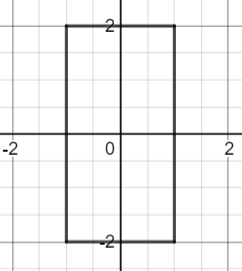
\includegraphics{resources/img/subgroup_example_rectangle_symmetries.png}
					\par
				\end{figure}
				These symmetry operations form a group whose group table is as follows.
				\begin{table}[h!]%
					\centering%
					\begin{tabular}{|c||c|c|c|c|}
						\hline
							&  $i$  & $a$   & $b$ & $c$ \\
						\hline
						\hline
						$i$ &  $i$  & $a$   & $b$ & $c$ \\
						\hline
						$a$ & $a$   & $i$ 	& $c$ & $b$ \\
						\hline
						$b$ & $b$ 	& $c$   & $i$ & $a$ \\
						\hline
						$c$ & $c$ 	& $b$ 	& $a$ & $i$ \\
						\hline
					\end{tabular}
				\end{table}
			}
		\end{exe}
	
		\bigskip
		\subsubsection{Cyclic Subgroups}
		\boxeddefinition{
			If we take a single member of a group (along with its inverse and the identity), the subgroup generated by that element takes the form (using multiplicative notation),
			\[ H = \{ x^{-(n-1)},\, \cdots , x^{-2}, x^{-1}, 1, x, x^2,\, \cdots , x^{n-1} \} \]
			where, either, $x^n = 1$ so that there are $n$ distinct values in the group, or else $n$ is infinite and the values never repeat.
			This is known as a \textbf{cyclic group} and also as the \textbf{subgroup generated by $\bm{x}$} and is denoted by $\langle x \rangle$.
		}
		\note{The cyclic subgroup, $\langle x \rangle$, generated by $x$ is the smallest subgroup of $G$ containing $x$ in the sense that, if ${ H \leq G }$ and ${ x \in H }$ then ${ \langle x \rangle \subseteq H }$.}
		
		\labeledProposition{Every cyclic group is Abelian.}{cyclic_groups_are_abelian}
		\begin{proof}
			In a cyclic group every element has the form ${ x^i }$ for ${ i \in \Z{} }$. So we have,
			\[ x^mx^n = x^{m+n} = x^nx^m \]
			for all elements ${ x^i }$ in the group.
		\end{proof}
		
		
		\labeledProposition{The set $S$ of integers $n$ such that $x^n = 1$ is a subgroup of $\Z{+}$.}{cyclic_powers_add_subgroup_integers}
		\begin{proof}
			If $x^m = 1$ and $x^n = 1$, then $x^{m+n} = x^mx^n = 1$ also so we have closure of addition. Since $x^0 = 1$, 0 is in the subgroup so we have an identity. Finally, for some $n$ in the subgroup, $x^n = 1 \iff x^{-n} = x^nx^{-n} = x^0 = 1$ so $n$ being in the subgroup implies that $-n$ is also in the subgroup and we have inverses.
		\end{proof}
		\begin{corollary}
			It follows from $S$ being a subgroup of $\Z{+}$ and from \autoref{prop:bZ_subgroup} that $S$ has the form $m\Z{}$ where $m$ is the smallest positive integer such that $x^m = 1$. Therefore, in $H$, the $m$ elements $1, x, x^2, \cdots , x^{m-1}$ are all different and any element in $H$ will simplify to one of them: for $n \in S$, $n = mq + r$ such that $x^n = (x^m)^qx^r = 1^qx^r = x^r$.
		\end{corollary}
	
		
		\bigskip
		\subsubsection{Order}
		
		\boxeddefinition{The \textbf{order} of a group $G$ is the number of distinct elements it contains. It is typically denoted $\vert G \vert$.\\
			An element of a group is said to have \textbf{order} $m$ (possibly infinity) if the cyclic subgroup it generates has order $m$. This means that $m$ is the smallest positive integer with the property $x^m = 1$ or, if the order is infinite, that, $x^m \neq 1$ for all $m \neq 0$.
		}
	
		\labeledTheorem{An element and its inverse have the same order.}{order_of_inverse_is_the_same}
		\begin{proof}
			Firstly we need to consider the case that an element $x$ has infinite order. In this case, ${ \nexists m \in \N{} \suchthat x^m = e }$. Now suppose that ${ \exists n \in \N{} \suchthat (\inv{x})^n = e }$. Then we have,
			\[ (\inv{x})^n = \inv{(x^n)} = e \iff e = x^n \]
			which contradicts the hypothesis that $x$ has infinite order. Therefore ${ \inv{x} }$ has infinite order also. Clearly also this argument can be used in reverse to show the reverse implication also holds.\\\\
			Now consider the case that $x$ has finite order. Let ${ x \in G }$ be an arbitrary member of an arbitrary group such that ${ x^m = e }$. Then ${ \inv{x} = x^{m-1} }$ and if we consider powers ${ i \in \N{} }$ of the inverse ${ (\inv{x})^i = (x^{m-1})^i }$ then the order is the lowest value of ${ i(m-1) }$ such that ${ x^{i(m-1)} = e }$. But we know that the lowest power of $x$ equal to $e$ is $m$ so we're looking for the lowest multiple of $m$ that has the form ${ i(m-1) }$. So we require,
			\[ m \divides i(m-1) = im - i \iff (m \divides im) \land (m \divides i) \]
			which clearly requires that ${ m \divides i }$. Also, clearly, the lowest such $i$ is ${ i = m }$.\\\\
			Another way to show this is to say that if ${ x^m = e }$ then,
			\[ (\inv{x})^m = \inv{(x^m)} = e \]
			so that the order of ${ \inv{x} }$ is less than or equal to $m$. Conversely, if ${ \inv{x} }$ has order $n$ then,
			\[ x^n = (\inv{(\inv{x})})^n = \inv{((\inv{x})^n)} = \inv{e} = e \]
			so that the order of ${ x }$ is less than or equal to $n$. Thus we have,
			\[ m \leq n,\; n \leq m \implies m = n. \]
		\end{proof}
	
		\labeledTheorem{An element has order 2 iff it is equal to its inverse.}{order_2_element_equal_to_inverse}
		\begin{proof}
			Let ${ x \in G }$ be an arbitrary member of an arbitrary group such that ${ x^2 = e }$. Then by \autoref{theo:order_of_inverse_is_the_same} we have,
			\[ e = x^2 = (\inv{x})^2 = x^{-2} \iff x = \inv{x}. \]
			Also,
			\[  x = \inv{x} \iff x^2 = e. \]
		\end{proof}
	
		\labeledTheorem{A group of finite order cannot have any element of infinite order.}{finite_group_no_infinite_order_element}
		\begin{proof}
			If $G$ is a group and ${ x \in G }$ has infinite order then,
			\begin{align*}
			&& x^m &= x^n \\
			&\iff & x^{m-n} &= 1= x^{n-m} &\sidecomment{} \\
			&\iff & x^{\abs{m-n}} &= 1 &\sidecomment{} \\
			&\therefore & \abs{m-n} &= 0. &\sidecomment{because order of x is infinite} \\
			\end{align*}
			So, there are no two distinct powers of $x$ that produce the same object so that ${ \langle x \rangle \leq G }$, the cyclic group generated by $x$, is infinite. Since ${ \langle x \rangle \subseteq G }$ this requires that $G$ also be infinite.
		\end{proof}
	
		\bigskip
		\labeledTheorem{If a group element $x$ has finite order $m$ then:
			\begin{enumerate}
				\item{Let ${ n \in \Z{}. }$ If ${ n = km + r }$ where ${ k,r \in \Z{} }$ and ${ 0 \leq r \leq m - 1 }$, then ${ x^n = x^r. }$}
				\item{For ${ n \in \N{},\; x^n = 1 \iff m | n. }$}
				\item{${ 1,x,x^2,\dots,x^{m-1} }$ is a complete, repetition-free, list of elements of ${ \langle x \rangle. }$}
				\item{The subgroup ${ \langle x \rangle }$ generated by $x$ has cardinality $m$.}
			\end{enumerate}
		}{finite_order_group_element_properties}
	
		\bigskip
		\labeledTheorem{In an Abelian group the set of all elements of finite order forms a subgroup.}{finite_order_elements_in_abelian_group_are_subgroup}
		\begin{proof}
			Let $S$ be the set of all elements of finite order,
			\[ S = \setc{g \in G}{\exists m \in \N{} \logicsep g^m = e}. \]
			\begin{itemize}
				\item{Firstly, $S$ is non-empty because it contains the identity.}
				\item{Secondly, if we have ${ a,b \in S }$ then ${ a^i = b^j = e }$ for some ${ i,j \in \N{} }$. Then, if we let ${ m = i \times j }$,
					\[ (ab)^m = a^mb^m = (a^i)^j(b^j)^i = e \]
					where ${ (ab)^m = a^mb^m }$ is valid \textit{only} because the group is Abelian.
				}
				\item{Lastly, $S$ contains all inverses because,
					\[ a^i = e \iff a^{i-1} = \inv{a} \iff (\inv{a})^i = (a^i)^{i-1} = e. \]
					Therefore ${ \inv{a} \in S }$.
				}
			\end{itemize}		
		\end{proof}
	
		\labeledTheorem{If every non-identity element of a group has order 2 then the group is Abelian.}{non_identity_elements_are_order_2_then_abelian}
		\begin{proof}
			Let ${ x,y \in G }$ be two arbitrary elements of order 2 of an arbitrary group. Then by \autoref{theo:order_of_inverse_is_the_same} we have ${ x = \inv{x},\; y = \inv{y},\; xy = \inv{xy} }$ and so,
			\[ xy = \inv{(xy)} = \inv{y}\inv{x} = yx. \]
			Note that ${ \inv{(xy)} = \inv{y}\inv{x} }$ relies only on the associativity of the group operation and is therefore valid for all groups.\\
			We can also show it this way,
			\[ (xy)^2 = e \iff xyxy = e \iff yxy = xe = x \iff yx = xy. \]
		\end{proof}
	
		\labeledTheorem{If a finite group has even-numbered order then it must have at least one element of order 2.}{even_ordered_group_has_element_of_order_2}
		\begin{proof}
			By the group properties we know that the group contains the identity element -- which has order 1 -- and, for every non-identity element, the group also contains its inverse. Also, since the group is finite, every element must have finite order. Now, if every non-identity element is distinct from its inverse then the order of the group will be odd (because of the identity and then every other element is paired with its inverse). For the group's order to be even we must have at least one non-identity element that is not distinct from its inverse which, by \autoref{theo:order_2_element_equal_to_inverse}, is equivalent to having order 2.
		\end{proof}
		\begin{corollary}
			If a finite group has even-numbered order then it must have an odd number of elements of order 2.
		\end{corollary}
		\begin{proof}
			Let $G$ be a finite group with even-numbered order and $M$ be the number of elements that are distinct from their inverse and $N$ be the number of elements that are not distinct from their inverse (these correspond to elements with order greater than 2 and elements with order 2 respectively). Then the order of $G$ can be expressed as,
			\[ \cardinality{G} = 1 + 2M + N. \]
			Therefore, ${ \cardinality{G} }$ is even if $N$ is an odd natural number.
		\end{proof}
	
		\labeledTheorem{In an infinite cyclic group all elements have infinite order.}{infinite_cyclic_group_elements_are_infinite_order}
		\begin{proof}
			Let ${ G = \langle x \rangle }$ be an infinite cyclic group. Suppose there is some non-identity element of $G$, ${ x^n }$ with finite order $m$. Then,
			\[ (x^n)^m = e \iff x^{nm} = e \]
			which contradicts the hypothesis that ${ \langle x \rangle }$ is infinite.
		\end{proof}
		\note{Note that the elements of an infinite cyclic group having infinite order does not mean that they generate the group. For example in an infinite cyclic group ${ \langle x \rangle }$, the element $x^2$ generates the cyclic subgroup,
			\[ \dots x^{-4}, x^{-2}, e, x^2, x^4, \dots \]
			which is infinite but clearly doesn't generate the whole group ${ \langle x \rangle }$.
		}
	
		\labeledTheorem{An infinite cyclic group has 2 generators.}{infinite_cyclic_group_has_2_generators}
		\begin{proof}
			Let ${ G = \langle x \rangle }$ be an infinite cyclic group and suppose there is some non-identity element of $G$, ${ x^n }$ that generates the group. To show this we only need to show that ${ x^n }$ can generate $x$ because, since $x$ is a member of the group, it is obviously necessary to generate it but, also, if we generate $x$ then we can generate all the other members of the group since they are powers of $x$.\\
			So let there be an integer $a$ such that ${ (x^n)^a = x^{an} = x \iff x^n = x^{1/a} }$. The cyclic group ${ \langle x \rangle }$ only contains integer powers of $x$ so it therefore follows that ${ \abs{a} = 1 }$ which implies that ${ n = 1 \text{ or } -1 }$ and ${ x^n = x \text{ or } \inv{x} }$.
			\note{We could also say that,
				\[ x^{an} = x \iff x^{an - 1} = e \]
				but this implies that the order of $x$ is finite and so contradicts the hypothesis that $x$ generates an infinite cyclic group.
			}
		\end{proof}
	
		\labeledTheorem{Let ${ G = \langle x \rangle }$ be a finite cyclic group of order $n$. If $r$ is a positive integer then ${ G = \langle x^r \rangle }$ if and only if the greatest common divisor of $n$ and $r$ is 1.}{coprime_order_element_generates_group}
		\begin{proof}
			Members of ${ \langle x^r \rangle }$ have the form ${ (x^r)^a }$ for some ${ a \in \Z{} }$. For integers ${ b,i }$,
			\[ (x^r)^a = x^{ar} = x^{bn + i} = x^{bn}x^i = ex^i = x^i \]
			so that the generated elements are ${ x^i }$ where ${ i = ar - bn }$ is the remainder when dividing $ar$ by $n$. If ${ d = gcd(n,r) }$ then ${ d \divides i }$ and the generated elements are powers of $x$ that are multiples of $d$. Therefore, to generate every power of $x$ it is necessary to have ${ d = 1 }$. Conversely, we can see -- by the same argument in reverse -- that it is sufficient if ${ d = 1 }$ to generate all the powers of $x$.\\\\
			Alternatively, we can say if ${ d > 1 }$ then ${ n/d }$ is a positive integer less than $n$ and ${ r/d }$ is a positive integer so,
			\[ (x^r)^{n/d} = (x^n)^{r/d} = e^{r/d} = e \]
			which shows that the order of $x^r$ is less than or equal to ${ n/d }$ which is less than $n$. Therefore the order of the cyclic group it generates is less than $n$ and so it cannot be equal to $G$.\\
			Conversely, if ${ d = 1 }$ then $n$ and $r$ are coprime and so we have,
			\[ (x^r)^m = e \iff x^{rm} = e \implies n \divides rm \implies n \divides m \implies m \geq n. \]
			This says that the order of ${ x^r }$ in $G$ is greater than or equal to $n$, the order of $G$. Well, clearly it cannot be greater than the order of $G$ so it follows therefore, that the order of $x^n$ is $n$. Since ${ \cardinality{\langle x^r \rangle} = \cardinality{G} }$ we can conclude that ${ \langle x^r \rangle = G }$.
		\end{proof}
	
		\labeledTheorem{A group $G$ is such that $G$ contains at least 2 elements and the only subgroups of $G$ are ${ \{e\} }$ and $G$ itself. Then $G$ is a finite cyclic group of prime order.}{no_proper_subgroups_implies_finite_cyclic_prime_ordered}
		\begin{proof}
			$G$ contains at least 2 elements so there is at least one non-identity element $x$. The only subgroups of $G$ are the whole group and ${ \{e\} }$ but ${ \langle x \rangle  }$ cannot equal ${ \{e\} }$ so it must equal $G$. Therefore $G$ is the cyclic group generated by $x$.\\
			But if $G$ were the infinite cyclic group generated by $x$ then only $x$ and $\inv{x}$ would generate the group and all other non-identity elements -- say $x^n$ for ${ n > 1 \in \N{} }$ -- would generate subgroups ${ \langle x^n \rangle \neq G }$. Therefore, $G$ cannot be infinite and is therefore finite.\\
			Now, we have a finite cyclic group where every non-identity element generates the group. Let ${ \cardinality{G} = n }$. Then, for every ${ m \suchthat 0 < m < n }$, ${ \langle x^m \rangle = G }$ and, by \autoref{theo:coprime_order_element_generates_group}, $m$ and $n$ are coprime. Therefore, $n$ is prime.\\
			Here we could also use a proof by contradiction: Assume $n$ is not prime and it has factors ${ r,s > 1 \in \N{} }$. Then,
			\[ (x^r)^s = x^{rs} = x^n = e \]
			so that the order of $x^r$ in $G$ is less than or equal to $s$ which is less than $n$ (because it is a factor of $n$). It follows then that ${ \langle x^r \rangle \neq G }$, contradicting the definition of $G$. Therefore $n$ is prime.
		\end{proof}
	
		\bigskip
		\labeledProposition{Suppose the elements ${ x,y }$ in a group $G$ have orders ${ m,n }$ respectively and that the ${ gcd(m,n) = 1 }$. Then ${ \langle x \rangle \cap \langle y \rangle = \{e\} }$ and, if $x$ and $y$ commute, then the order of $xy$ in $G$ is $mn$.}{coprime_order_elements_have_disjoint_cyclic_groups}
		\begin{proof}
			One way to approach this is to say that for ${ z \in \langle x \rangle \cap \langle y \rangle }$ we have some ${ 0 \leq i < m, 0 \leq j < n }$ such that,
			\[ z = x^i = y^j \iff x^{im} = e = y^{jm},\, x^{in} = y^{jn} = e \]
			so that ${ x^{in} = y^{jm} = e \iff (m \divides in \eqand n \divides jm) }$. Note that,
			\[ (m \divides in \eqand n \divides jm) \iff m,n \divides in + jm. \]
			Now, applying the fact that ${ gcd(m,n) = 1 }$ we see that both $m$ and $n$ must divide 1. But both $m$ and $n$ are orders of elements and so, by definition, greater than 1. The only other alternative is that both ${ i,j = 0 }$ which results in ${ z = x^0 = y^0 = e }$.\\
			
			We could also have said,
			\[ x^{im} = e = x^{in} \iff x^{im - in} = e \iff m \divides im - in. \]
			In this case we can apply the fact that ${ gcd(m,n) = 1 }$ to the statement that ${ m \divides i(m-n) }$ to deduce that: either ${  m \divides (m-n) \iff m \divides 1 }$ which is impossible because $m$ must be greater than 1; or ${ m \divides i }$ which is also impossible because ${ i < m }$. So, again, we are only left with the alternative that ${ i = 0 }$ which results in ${ z = x^0 = y^0 = e }$.\\
			
			Next we prove the order of ${ xy \in G }$ and we begin by noting that, if $x$ and $y$ commute, then ${ (xy)^r = x^ry^r }$. So if we assume that $xy$ has order $r$ then we must have ${ m,n \divides r }$ and the lowest such $r$ is the order. Well, the lowest common multiple of ${ m,n }$ is defined according to the gcd as described in the Number Theory treatment of Modular Arithmetic (\ref{sssec:lowest_common_multiple}) as,
			\[ d = gcd(m,n) \implies lcd(m,n) = d \cdot (m/d) \cdot (n/d). \]
			Clearly then, if ${ d = gcd(m,n) = 1 }$, then the lowest common multiple is ${ mn }$ and so the order of ${ xy \in G }$ is ${ mn }$.\\
			
			Or to describe it a different way: ${ (xy)^{mn} = x^{mn}y^{mn} = ee = e }$ so that the order of $xy$,
			\[ \cardinality{xy} \leq mn. \]
			Conversely any $r$ such that ${ (xy)^r = e }$ must have ${ m,n \divides r }$ and the lowest common multiple of $m$ and $n$ is $mn$ so
			\[ r \geq mn. \]
			Therefore, ${ \cardinality{xy} = mn }$.			
		\end{proof}
	
		\bigskip
		\subsubsection{Examples of Cyclic Subgroups}
		\bigskip
		\begin{exe}
			\ex{\textbf{Cyclic group with order 3}
				\[ G = \{1, x, x^2\} \]
				where $x^3 = 1$ is a cyclic group of order 3 generated by the element $x$. Note that, since this is a group, it must also contain the inverses, $x^{-1}, x^{-2}$ but ${ x^3 = 1 }$ so ${ x^{-1} = x^2 }$ and ${ x^{-2} = x }$.\\
			}
			\ex{\textbf{Symmetries of an equilateral triangle}\\\\
				Consider an equilateral triangle with vertices labeled ${ A,B,C }$:
				\begin{align*}
		  		& A &  \\
				B & \hspace{7pt} C. & \\
				\end{align*}
				Every permutation of the vertices is a transformation that produces an object that occupies the same space as the original, i.e. a \textit{symmetry}. If we take one of them, say, the clockwise rotation one place that results in,
				\begin{align*}
				& B &  \\
				C & \hspace{7pt} A & \\
				\end{align*}
				and we name this $r$, then clearly -- since there are 3 vertices -- performing this same rotation 3 times leaves us back where we started. So, using function composition as the law of composition and multiplicative notation, $r^3 = i$ where $i$ is the identity transformation. Also the inverse of $r$ is $r^2$. So, we have a group consisting of ${ \{i, r, r^2\} }$ and function composition. Notice the resemblance of this group to the previous group ${ \{1, x, x^2\} }$; this group is \textit{isomorphic} to the cyclic group of order 3.\\
			}
			\ex{\textbf{Group ${\bm{ (\Z{*}_5, \otimes) }}$}\\\\
				Consider the element 2 modulo 5. Using multiplicative notation we have,
				\[ 2^2 = 4, 2^3 = 8 = 3, 2^4 = 16 = 1, 2^5 = 32 = 2. \]
				So ${ 2^1 = 2^5 \iff 1 = 2^4 }$ meaning that the element 2 has order 4 in the group and we see, as expected that the group it generates, ${ \langle 2 \rangle }$ has 4 members. In this case, the members are all the members of the group -- that's to say, \textit{the element 2 generates the whole group}. If we consider the element 4 we have,
				\[ 4^2 = 16 = 1, 4^3 = 64 = 4. \]
				So this element oscillates between 1 and 4 and so, the cyclic subgroup that it generates ${ \langle 4 \rangle }$ has order 2.\\
				Since the group ${ (\Z{*}_5, \otimes) = \langle 2 \rangle }$ it can also be described as a cyclic group. This will be the case for any such group modulo a prime number -- i.e. ${ (\Z{*}_p, \otimes) }$ where $p$ is prime.\\
			}
			\ex{\textbf{Cyclic group with infinite order}
				\[
				\begin{bmatrix}
				1 & 1	\\
				0 & 1 	\\
				\end{bmatrix} 
				\]
				under matrix multiplication (which is commutative in this case), generates a cyclic group of infinite order because
				\[
				\begin{bmatrix}
				1 & 1	\\
				0 & 1 	\\
				\end{bmatrix}^n =
				\begin{bmatrix}
				1 & n	\\
				0 & 1 	\\
				\end{bmatrix}.
				\]
				\smallskip
			}
			\ex{\textbf{Cyclic groups in a non-Abelian group}\\\\
				Consider the following two elements in ${ GL(2,\R{}) }$,
				\[
					A = \begin{pmatrix}
					0  & 1 \\
					-1 & 0
					\end{pmatrix},\hspace{10pt}
					B = \begin{pmatrix}
					0 & -1 \\
					1 & -1
					\end{pmatrix}.
				\]
				Both of these elements have finite order as,
				\[
					(A^2)^2 =
					\begin{pmatrix}
					-1  & 0 \\
					0   & -1
					\end{pmatrix}^2 =
					\begin{pmatrix}
					1  & 0 \\
					0  & 1
					\end{pmatrix},
				\]
				\[
					(B^2)B =
					\begin{pmatrix}
					-1  & 1 \\
					-1  & 0
					\end{pmatrix}
					\begin{pmatrix}
					0  & -1 \\
					1  & -1
					\end{pmatrix} =
					\begin{pmatrix}
					1  & 0 \\
					0  & 1
					\end{pmatrix}.
				\]
				But their product $AB$ does not have finite order.
				\[
					AB =
					\begin{pmatrix}
					1  & -1 \\
					0  & 1
					\end{pmatrix},\hspace{10pt}
					(AB)^n =
					\begin{pmatrix}
					1  & -1 \\
					0  & 1
					\end{pmatrix}^n =
					\begin{pmatrix}
					1  & -n \\
					0  & 1
					\end{pmatrix}
				\]
				for any ${ n \in \N{} }$.
				\bigskip
			}
			\ex{\textbf{The Klein Four Group, $V$} is the simplest group that is not cyclic (it cannot be generated by a single element). It appears in many forms but, as an example, it can be realized as the group consisting of the four matrices,
				\[
				\begin{bmatrix}
				\pm 1 & 0 		\\
				0 & \pm 1 	\\
				\end{bmatrix} 
				\]
				Any two non-identity elements generate $V$.
			}
		\end{exe}
	}

	
	\pagebreak
	\searchableSubsection{Isomorphisms}{abstract algebra}{\bigskip
		\boxeddefinition{An \textbf{isomorphism} is a bijection between two groups that preserves the structure of the groups by being compatible with the law of composition of both groups. More formally, two groups are \textbf{isomorphic} if there exists a bijection $\phi : G \longmapsto G'$ such that,
			\[ \phi(ab) = \phi(a)\phi(b) \text{ for all } a,b \in G \]
			where $ab$ represents composition according to the law of composition of $G$ and $\phi(a)\phi(b)$ represents composition according to the law of composition of $G'$.
		}
	
		\note{An \textbf{isomorphism} is a \textbf{bijection} between two \textbf{groups}. That's to say, it is already assumed in the definition of an isomorphism that the codomain $G'$ is a group.}
	
		\labeledProposition{As a consequence of this sole property that, across the bijection, the respective laws of composition are preserved, all other properties of the groups are also preserved.}{isomorphism_preserves_structure}
		\begin{proof}
			Let $e$ be the identity in $G$ and $e' = \phi(e) \in G'$, and $1'$ be the identity element in $G'$ then,
			\begin{itemize}
				\item{
					Since $G'$ is a group, it has the inverses property that every element has an inverse so,
					\begin{align*}
						 &&e' &= \phi(e) = \phi(ee) = \phi(e)\phi(e) = e'e' &\sidecomment{using preservation of law of composition}\\
						 &\iff &\inv{(e')}e' &= (\inv{(e')}e')e' &\sidecomment{using the inverses property of $G'$}\\
						 &\iff &1' &= e'
					\end{align*}
					which implies that $e'$ is the identity in $G'$ so that $\phi$ maps the identity in $G$ to the identity in $G'$.}
				\item{We can use the fact just shown that $\phi(e) = e' = 1'$ to show,
					\begin{align*}
						&&1' = e' = \phi(e) &= \phi(a\inv{a}) = \phi(a)\phi(\inv{a}) &\sidecomment{using preservation of law of composition}\\
						&\iff &\inv{\phi(a)}1' &= \inv{\phi(a)}\phi(a)\phi(\inv{a}) &\sidecomment{using the inverses property of $G'$}\\
						&\iff &\inv{\phi(a)} &= \phi(\inv{a})
					\end{align*}
					which shows that $\phi$ maps $\inv{a} \in G$ to $\inv{\phi(a)} \in G'$.}
			\end{itemize}
		\end{proof}
		
		 For example, if $e \in G$ is the identity of $G$ mapped to an element $ e' = \phi(e) \in G' $, then for any $a \in G$ mapped to $a' = \phi(a) \in G'$,
		\[ a' = \phi(a) = \phi(ea) = \phi(e)\phi(a) = e'a' \]
		And $a' = e'a' = a'e'$ means that $e'$ is the identity in $G'$. Furthermore, the order of elements in $G$ and $G'$ will also be the same as,
		\[ a^n = e \iff e' = \phi(e) = \phi(a^n) = \phi(a)^n = (a')^n \]
		
		Since two isomorphic groups have the same properties, it is often convenient to identify them with each other when speaking informally. For example, the symmetric group $S_n$ of permutations of $\{1,\cdots,n\}$ is isomorphic to the group of permutation matrices, a subgroup of $GL_n(\R{})$ and we often blur the distinction between these two groups.\\
		
		\notation{Sometimes when two groups are isomorphic this is indicated using the notation,
			\[G \approx G'\]
		}
	
		\subsubsection{Examples}
		\begin{itemize}
			\item{
				Let $C = \{ \cdots, a^{-2}, a^{-1}, 1, a, a^2, \cdots \}$ be an infinite cyclic group. Then the map,
				\[ \phi : \Z{+} \longmapsto C \; \suchthat \; \phi(n) = a^n \]
				is an isomorphism where the preservation of the respective laws of composition can be seen as,
				\[ \phi(m + n) = a^{m + n} = a^ma^n = \phi(m)\phi(n) \]
				and also ${ n + (-n) = 0 }$ and,
				\[ \phi(-n) = a^{-n} = \inv{(a^n)}. \]
			}
			\item{Let $G$ be the set of real matrices of the form,
				\[
				\begin{bmatrix}
				1 & x 	\\
				0 & 1 	\\
				\end{bmatrix} 
				\]
				This is a subgroup of $GL_2(\R{})$ and so, its law of composition is the same as that of $GL_2(\R{})$, i.e. matrix multiplication.
				\[
				\begin{bmatrix}
				1 & x 	\\
				0 & 1 	\\
				\end{bmatrix}
				\begin{bmatrix}
				1 & y 	\\
				0 & 1 	\\
				\end{bmatrix} = 
				\begin{bmatrix}
				1 & x + y\\
				0 & 1 	\\
				\end{bmatrix}
				\]
				So, $G$ is isomorphic to $\R{+}$, the additive group of reals.
			}
		\end{itemize}
		
		\boxeddefinition{The groups isomorphic to a given group $G$ form what is called the \textbf{isomorphism class} of $G$. Groups are often classified into isomorphism classes, for example, there is one isomorphism class of groups of order 3 and there are two classes of groups of order 4 and five classes of 12.}
		
		\labeledProposition{There is only one isomorphism class for each order of cyclic group.}{one_class_per_cyclic_order}
		\begin{proof}
			Any two cyclic groups of the same order are isomorphic because, if
			\[ G = \{1, x, x^2, \cdots, x^{n-1}\}, \; G' = \{1, y, y^2, \cdots, y^{n-1}\} \]
			are two cyclic groups of order $n$ then the map $\phi(x^i) = y^i$ is an isomorphism.
		\end{proof}
	
		\medskip
		\labeledProposition{\textbf{Cayley's Theorem} states that every group is isomorphic to a group of permutations of the same underlying set, or in other words, to a subgroup of the symmetric group acting on the group.}{cayleys_theorem}
		\begin{proof}
			Let $G$ be a group and ${ x \in G }$ and define ${ f_x : G \longmapsto G }$ as ${ f_x(g) = xg }$. Then $f_x$ is a bijection because it has an inverse ${ \inv{f_x}(g) = \inv{x}g = f_{\inv{x}}(g) }$. Therefore $f_x$ is a permutation.\\
			
			Now we define a map, from $G$ to the symmetric group of permutations of $G$, that maps each element $x$ in $G$ to the permutation defined by $f_x$. Let ${ \phi: G \longmapsto Sym(G) }$ be defined as ${ \phi(x) = f_x }$ then,
			\begin{itemize}
				\item{$\phi$ is homomorphic because
					\[ (f_x \circ f_{x'})(g) = f_x(f_{x'}(g)) = x(x'g) = xx'g = f_{xx'}(g) \]
					and so,
					\[ \phi(xx') = f_{xx'} = f_x \circ f_{x'} = \phi(x) \circ \phi(x'). \]
				}
				\item{$\phi$ is injective because if ${ x,x' \in G }$ such that ${ x \neq x' }$ then ${ f_x(e) = x \neq x' = f_{x'}(e) }$ is sufficient to show that ${ f_x \neq f_{x'} }$. Or alternatively, the kernel of $\phi$ comprises the elements ${ k \in G }$ such that ${ f_k(g) = kg = g \iff k = e }$ so that the kernel is the trivial subgroup ${ \{e\} }$.
				}
			\end{itemize}
			Since $\phi$ is homomorphic, its image ${ im\,\phi }$ is a subgroup of ${ Sym(G) }$ and since $\phi$ is injective, it is in bijective correspondence with its image ${ im\,\phi \leq Sym(G) }$.\\
			Therefore $G$ is isomorphic to a subgroup of $Sym(G)$.
		\end{proof}
		
		\bigskip
		\subsubsection{Automorphisms}
		\boxeddefinition{The domain and codomain of an isomorphism can be the same set of objects so that $\phi : G \longmapsto G$. This is known as an \textbf{automorphism}.}
		\paragraph{Example}
		Let $G = \{1, x, x^2\}$ be a cyclic group of order 3 so that $x^3 = 1$. The transposition which interchanges $x$ and $x^2$ is an automorphism of $G$,
		\[\begin{array}{*6c}
			&1 &&\longmapsto &&1 \\
			&x &&\longmapsto &&x^2 \\
			&x^2 &&\longmapsto &&x \\
		\end{array}\]
		\begin{table}[h!]%
			\centering%
			\begin{tabular}{|c||c|c|c|}
				\hline
				      &  1    & $x$   & $x^2$ \\
				\hline
				\hline
				 1    &  1    & $x$   & $x^2$ \\
				\hline
				$x$   & $x$   & $x^2$ & 1     \\
				\hline
				$x^2$ & $x^2$ & 1     & $x$ \\
				\hline
			\end{tabular}
			$ \longmapsto $
			\begin{tabular}{|c||c|c|c|}
				\hline
				      &  1    & $x^2$ & $x$  \\
				\hline
				\hline
				1     &  1    & $x^2$  & $x$  \\
				\hline
				$x^2$ & $x^2$ & $x$   & 1    \\
				\hline
				$x$   & $x$   & 1     & $x^2$ \\
				\hline
			\end{tabular}
		\end{table}
		\\\\This is because the group is cyclic and $x$ and $x^2$ have the same order ($x^3 = 1$ and also $(x^2)^3 = x^6 = (x^3)^2 = 1^2 = 1$). So the law of composition is preserved.
		
		\bigskip
		\subsubsection{Conjugation}
		The most important example of automorphism is conjugation.\\\\
		\boxeddefinition{\textbf{Conjugation} by $b \in G$ is the map from $G$ to itself defined by,
			\[ \phi(a) = ba\inv{b} \]
			with the result that,
			\[ ba = \phi(a)b \]
			so that we can think of conjugation of $a$ by $b$ as the way that we need to change $a$ if we want to move the multiplication by $b$ to the other side.
		}
		This is an automorphism (known as an \textit{inner automorphism}) because it
		\begin{itemize}
			\item{is compatible with law of composition, 
				\[ \phi(xy) = bxy\inv{b} = bx\inv{b}by\inv{b} = \phi(x)\phi(y). \]
			}
			\item{has an inverse so it is bijective, 
				\[ (\inv{\phi} \circ \phi)(a) = \inv{\phi}(\phi(a)) = \inv{b}(ba\inv{b})b = (\inv{b}b)a(\inv{b}b) = a. \]
				Note that this is different from the inverse element of $a$ corresponding under the mapping $\phi$,
				\[ \phi(a)\phi(\inv{a}) = ba\inv{b}b\inv{a}\inv{b} = ba(1)\inv{a}\inv{b} = b(1)\inv{b} = 1. \]
			}
		\end{itemize}
		A couple more important properties of the conjugate are as follows.
		\begin{enumerate}[label=(\roman*)]
			\item{In an abelian group where the composition law is commutative, conjugation becomes the identity map.
				\[ ba = ab \iff ba\inv{b} = a \iff \phi(a) = a. \]}
			\item{The inverse of the conjugate ${ ba\inv{b} = \inv{b}ab }$.}
		\end{enumerate}
	}

	
	\bigskip\bigskip
	\searchableSubsection{Homomorphisms}{abstract algebra}{\bigskip
		\boxeddefinition{A \textbf{homomorphism} is a mapping (not necessarily bijective) between two groups, $\phi : G \longmapsto G'$, such that,
			\[ \phi(ab) = \phi(a)\phi(b) \text{ for all } a,b \in G \]
			where $ab$ represents composition according to the law of composition of $G$ and $\phi(a)\phi(b)$ represents composition according to the law of composition of $G'$. 
		}
		So, the difference between a \textit{homomorphism} and a \textit{isomorphism} is that the latter is bijective whereas the former is not. As a result, a \textit{homomorphism} may be one-way only.\\
		
		\note{A \textbf{homomorphism} is a \textbf{mapping} between two \textbf{groups}. That's to say, it is already assumed in the definition of a homomorphism that the codomain $G'$ is a group.}
		
		\paragraph{Examples of homomorphisms}
		\begin{exe}
			\ex {	Let $C = \{ a^{n-1}, \cdots, a^{-2}, a^{-1}, 1, a, a^2, \cdots, a^{n-1} \}$ be a finite cyclic group. Then the map,
				\[ \phi : \Z{+} \longmapsto C \; \suchthat \; \phi(n) = a^n \]
				is a homomorphism. Note that if $C$ were an infinite cyclic group then this would be an isomorphism. }\label{ex_finite_cyclic_group}
			\ex {the sign of a permutation $ sign : S_n \longmapsto {\pm1} $}\label{ex_sign_permutation}
			\ex {the determinant function $ det : GL_n(\R{}) \longmapsto \R{\times} $}\label{ex_determinant}
			\ex {an arguably trivial example is called the \textit{inclusion} map $i : H \longmapsto G$ of a subgroup $H$ into a group $G$, defined by $i(x) = x$. It functions as the identity for elements in the subgroup $H$ but, since it is not surjective, there is no inverse mapping.}\label{ex_inclusion_map}
		\end{exe}
	
		
		
		\subsubsection{Image of a homomorphism}\label{sssection:image_of_homomorphism}
		Since a homomorphism is not bijective it has an image different to the codomain group,
		\[ im \; \phi = \setc{x \in G'}{\exists a \in G \suchthat \phi(a) = x} \]
		The image of a homomorphism is a subgroup of the codomain group $G'$ because the homomorphism preserves the group structure as described in \autoref{prop:isomorphism_preserves_structure}.\\\\
		\notation{The image of the mapping $\phi$ with domain $G$ is sometimes denoted $\phi(G)$.}
		
		\subsubsection{Kernel of a homomorphism}
		\boxeddefinition{The \textbf{kernel} of a homomorphism is the set of elements in the domain that are mapped to the identity,
			\[ ker \; \phi = \setc{a \in G}{\phi(a) = 1'} \]
		}
	
		\labeledProposition{The kernel of a homomorphism is a subgroup of the domain group $G$.}{homomorphism_kernel_subgroup}
		\begin{proof}
			If $a,b \in ker \; \phi$ then,
			\begin{itemize}
				\item{closure: $ \phi(ab) = \phi(a)\phi(b) = 1' \cdot 1' = 1' $ which shows that 
					\[ a,b \in ker \; \phi \implies ab \in ker \; \phi. \] }
				\item{identity: By \autoref{prop:isomorphism_preserves_structure}, $ 1' = e' = \phi(e) $ and so $e \in ker \; \phi $.}
				\item{inverses: Since $ a \in ker \; \phi $, then 
					\begin{align*}
					&&1' = e' &= \phi(e) = \phi(a\inv{a}) = \phi(a)\phi(\inv{a}) = 1'\phi(\inv{a}) \\
					&\iff &1' &= \phi(\inv{a})
					\end{align*}
					so that $ a \in ker \; \phi \iff \inv{a} \in ker \; \phi $.}
			\end{itemize}
		\end{proof}
	
		\labeledProposition{If $\phi : G \longmapsto G'$ is a group homomorphism with kernel $N$ then, for $a,b \in G$,
			\[\phi(a) = \phi(b) \iff \exists n \in N, \suchthat b = an  \]
			or, equivalently, $\inv{a}b \in N$.
		}{kernel_elements_relate_congruent_elements}
		\begin{proof}
			\begin{align*}
			&& b &= an  \\
			&\implies & \phi(b) &= \phi(an) \\
			&\implies & \phi(b) &= \phi(a)\phi(n) &\sidecomment{by homomorphism property} \\
			&\implies & \phi(b) &= \phi(a)1' &\sidecomment{n is in the kernel} \\
			&\implies & \phi(b) &= \phi(a) \\
			\end{align*}
			\begin{align*}
			&& \phi(b) &= \phi(a) \\
			&\implies & \inv{\phi(a)}\phi(b) &= 1'  &\sidecomment{codomain is a group so has inverses} \\
			&\implies & \phi(\inv{a})\phi(b) &= 1' &\sidecomment{by \autoref{prop:isomorphism_preserves_structure}} \\
			&\implies & \phi(\inv{a}b) &= 1' &\sidecomment{by homomorphism property} \\
			&\implies & \inv{a}b &= n \in N \\
			&\implies & b &= an \\
			\end{align*}
		\end{proof}
		
		\labeledTheorem{A homomorphism is injective iff its kernel is the trivial subgroup ${ \{e\} }$.}{homomorphism_injective_iff_kernel_is_trivial}
		\note{When asked to prove the proposition that a homomorphism is injective iff its kernel is the trivial subgroup ${ \{e\} }$, it's tempting to begin proving each direction of the bidirectional implication with a proof by contradiction (e.g. "Assuming there is a non-identity element in the kernel...") but the direct positive proof can be made very quick and simple with the above corollary.
		}
		\begin{proof}
			Let ${ \phi: G \longmapsto G' }$ be a homomorphism.\\\\
			Assume that $\phi$ is injective and ${ k \in ker\,\phi }$. Remembering that we always at least have ${ e_G \in ker\,\phi }$,
			\[ \phi(k) = e_{G'} = \phi(e_G) \iff k = e_G \]
			where the last implication is by the injectivity of $\phi$.\\\\
			Now assume that ${ ker\,\phi = \{e_G\},\, a,b \in G }$. Then,
			\begin{align*}
			&& \phi(a) &= \phi(b) &  \\
			&\iff & \phi(a)\inv{\phi(b)} &= e_{G'} & \\
			&\iff & \phi(a)\phi(\inv{b}) &= \phi(a\inv{b}) = e_{G'} &\sidecomment{using homomorphism properties} \\
			&\iff & a\inv{b} &\in ker\,\phi &\sidecomment{} \\
			&\iff & a\inv{b} &= e_G &\sidecomment{by assumption ${ ker\,\phi = \{e_G\} }$} \\
			&\iff & a &= b.  &\qedhere \\
			\end{align*}		
		\end{proof}
		
		\begin{corollary}
			A homomorphism is an isomorhpism if its kernel contains only the identity and its image is the whole of the codomain (i.e. it's surjective). 
		\end{corollary}
	
		\subsubsection{Examples of Kernels of Homomorphisms}
		\begin{exe}
			\ex The determinant function \ref{ex_determinant}, $ det : GL_n(\R{}) \longmapsto \R{\times} $, has a kernel,
			\[ \setc{\text{real $n\times n$ matrices $A$}}{det \, A = 1}, \]
			which is a subgroup of $GL_n(\R{})$ known as the \textit{special linear group} $SL_n(\R{})$.
			\label{ex_special_lin_group}
			\ex The sign of a permutation \ref{ex_sign_permutation} has a kernel that is the set of \textit{even} permutations,
			\[ A_n = \{\text{even permutations}\}, \]
			which is a subgroup of the symmetric group $S_n$ and is known as the \textit{alternating group}, $A_n$.
			\label{ex_alternating_group}
			\ex The map from the additive group of integers to a finite cyclic group \ref{ex_finite_cyclic_group},
			\[ \phi : \Z{+} \longmapsto C \; \suchthat \; \phi(n) = a^n \]
			has the kernel,
			\[ ker \; \phi = \setc{n \in \Z{+}}{a^n = 1} \]
			which has been proven to be a subgroup in \autoref{prop:cyclic_powers_add_subgroup_integers}.
			\label{ex_kernel_cyclic_powers}
		\end{exe}
	}


	\bigskip\bigskip
	\searchableSubsection{Equivalence Relations and Partitions}{abstract algebra}{\bigskip
		\notation{In the following treatment of equivalence relations we will use the notation $a \sim b$ to denote the equivalence of $a$ and $b$; $\overline{a}$ to indicate the equivalence class of $a$; and $\overline{S}$ to indicate the partition of $S$ comprised of equivalence classes such as the class $\overline{a} = \overline{b}$ which includes both $a$ and $b$.}
		Any map of sets $\phi: S \longmapsto T$ defines an equivalence relation on the domain $S$ such that $a \sim b$ iff $\phi(a) = \phi(b)$. We will refer to this as the \textit{equivalence relation determined by the map}. The corresponding partition is made up of the sets of elements in the domain $S$ that are mapped to the same element in the codomain $T$.\\\\
		\label{def:inverse_image}
		\boxeddefinition{Let $\phi: S \longmapsto T$ be a map, then the \textbf{inverse image} of an element $t \in T$ is defined as,
			\[ \inv{\phi}(t) = \setc{s \in S}{\phi(s) = t} \]
			and can also be applied to a set $U \in T$ as,
			\[ \inv{\phi}(U) = \setc{s \in S}{\phi(s) \in U} \]
			Note that in this notation, $\inv{\phi}$ \textbf{does not indicate an inverse function} as the inverse of the function may not exist but the inverse image is nevertheless defined.\\
			The inverse images - the sets $\inv{\phi}(t)$ for all $t \in T$ - may also be called the \textbf{fibres} of the map $\phi$.
		}
		Clearly, the non-empty fibres of the map $\phi$ form a partition of $S$. We can express this partition of $S$ as a bijection, that we shall call $\overline{\phi}$, between the fibres of $\phi$ in $S$ and the element of the image of $S$ to which their members are mapped,
		\[ \overline{\phi}: \overline{S} \longmapsto im \; \phi \]
		so that,
		\[ \overline{\phi}(\overline{s}) = \phi(s). \]
		
		\begin{figure}[h!]
			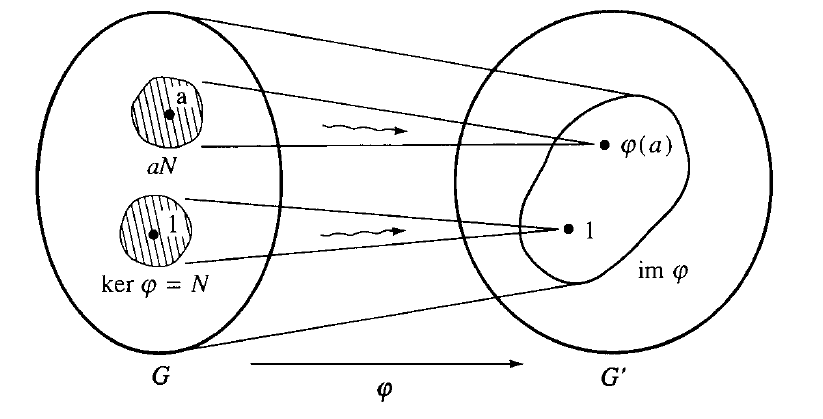
\includegraphics[width=\linewidth]{resources/img/group_homomorphism_schematic.png}
			\caption{A schematic diagram of a group homomorphism}
		\end{figure}
	
		\subsubsection{Congruence}
		Since a homomorphism maps the identity to the identity and inverses to inverses (\autoref{prop:isomorphism_preserves_structure}), we can deduce that the inverse image of the identity in $G'$ is going to contain at least the identity of $G$ and that the inverse image of an element $\inv{(a')} \in G'$ will contain at least the element $\inv{a} \in G$. So, in terms of equivalence classes we can say that, for a homomorphism $\phi$,
		\[ 1 = e \in \inv{\phi}(1') \implies \overline{\phi}(\overline{1}) = 1' \]
		\[ \inv{a} \in \inv{\phi}(\inv{(a')}) \implies \overline{\phi}(\overline{\inv{a}}) = \inv{(a')} \]

		\boxeddefinition{The equivalence relation determined by a homomorphism is known as \textbf{congruence} and is commonly denoted using $\equiv$ instead of $\sim$. For a homomorphism $\phi$,
			\[ a \equiv b \iff \phi(a) = \phi(b). \]
			Since $\phi$ is a homomorphism we also have,
			\[ a \equiv b \iff \phi(ac) = \phi(bc), \; \phi(\inv{a}) = \phi(\inv{b}). \]
			More generally, a \textbf{congruence relation} is an equivalence relation on an algebraic structure (such as a group, ring, or vector space) that is compatible with the structure in the sense that algebraic operations done with equivalent elements will yield equivalent elements.
		}
		\subsubsection{Congruence Examples}
		\begin{exe}
			\ex{The modulus function of complex numbers forms a homomorphism from the multiplicative group of complex numbers to the multiplicative group of reals,
				\[ \phi : \C{\times} \longmapsto \R{\times} \suchthat \phi(a) = \abs{a} \]
				and the induced equivalence relation is $a \equiv b \iff \abs{a} = \abs{b}$. The fibres of this map are the concentric circles about 0. They are in bijective correspondence with elements of $im \; \phi$, the set of positive reals.
			}\label{ex:modulus_of_complex_numbers_as_homomorphism}
		\end{exe}
	}

	
	\pagebreak
	\searchableSubsection{Cosets}{abstract algebra}{\bigskip
		The set of elements of the form $an$ - described in \autoref{prop:kernel_elements_relate_congruent_elements} - is denoted by $aN$ and is called a \textit{coset} of $N$ in $G$.\\\\
		\boxeddefinition{A coset can be defined for any subgroup $H$ of a group $G$. A \textbf{left coset} is a subset of the form,
			\[ aH = \setc{ah}{h \in H}. \]
		}
		\note{Cosets are not, in general, subgroups. This can be easily seen as the left coset $aH$ does not contain the identity as, although $H$ contains the identity, $aH$ contains ${ a1 = a }$.} 
		
		Note that the arbitrary subgroup $H$ could also be thought of as a coset $1H = H$ and also that the left cosets $aH$ are equivalence classes for the congruence relation,
			\[ a \equiv b \iff b = ah, \; h \in H. \]
		This is a congruence because, for some arbitrary $c \in G$,
			\[ 1 \equiv c \iff \exists h \in H \suchthat c = 1h = h. \]
		That's to say, the elements that are congruent to the identity are precisely the members of the subgroup $H$ so that it plays a similar role to the kernel $N$ in \autoref{prop:kernel_elements_relate_congruent_elements}. Furthermore, since the congruence relation is an equivalence relation it forms a partition of the domain $G$.
		
		\labeledProposition{For a group $G$ with a subgroup $H$ and ${ x \in G }$, the coset $xH$ is equal to $H$ iff ${ x \in H }$.}{coset_of_subgroup_member_is_subgroup}
		\begin{proof}
			Assume ${ x \in H }$. Then ${ \forall xh \in xH \logicsep xh \in H }$. Therefore ${ xH \subseteq H }$. Conversely, ${ \inv{x} \in H }$ so,
			\[ \forall h \in H \logicsep \inv{x}h \in H \implies x(\inv{x}h) = h \in xH. \]
			Therefore ${ H \subseteq xH }$ and so ${ H = xH }$.\\
			
			Now assume that ${ H = xH }$. Since ${ e \in H }$ then ${ xe = x \in xH = H }$ and so ${ x \in H }$.
		\end{proof}
		
		\labeledProposition{The left cosets of a subgroup partition the group.}{cosets_partition_group}
		\begin{proof}
			The left cosets are equivalence classes and, as a result, they partition the group.
		\end{proof}
	
		\subsubsection{Examples of cosets}
		\begin{exe}
			\ex{The coset of an element with the kernel $N$,
				\[ aN = \setc{g \in G}{g = an, \; n \in N} \]
				is the set of all elements that are \textit{congruent} to $a$. The \textit{congruence classes} are precisely the cosets $aN$ for each $a \in G$. They are also the nonempty \textit{fibres} of the homomorphic map.\medskip
			}\label{ex:coset_with_kernel}
			\ex \ref{S_3} Continuing the example of the symmetric group $S_3$ represented as 
				\[ G = \{1, x, x^2, y, xy, x^2y\} \]
				with group multiplication rules, 
				\[ x^3 = 1, y^2 = 1, yx = x^2y. \]
				The element $xy$ has order 2 so it generates a cyclic subgroup $H = \{1, xy\}$ of order 2. The left cosets of $H$ in $G$ are the three sets,
				\[ \{1,xy\} = 1H = xyH, \; \{x, x^2y\} = xH = x^2yH, \; \{x^2, y\} = x^2H = yH. \]
				Note that they do partition the group $G$. Also, notice that the cosets $aH$ for $a \in H$ produce the subgroup $H$ itself as should be expected as the group properties of the subgroup dictate that all products of its elements are already present in the subgroup. For this reason, the cosets $aH$ that are distinct from $H$ are those such that $a \not\in H$.\medskip\label{ex_S_3}
			\ex{Let ${ G = (\R{3}, +) }$ be the group of 3d vectors with vector addition and ${ \V{w} \in G }$. Then if
				\[ H = \setc{ \V{x} \in G }{ \V{w}^T\V{x} = \V{0} } \]
				then $H$ is a subgroup, ${ H \leq G }$. $H$ is a vector space representing a plane through the origin in $\R{3}$ and it's cosets are
				\[ \V{v} + H = \setc{ \V{v} + \V{h} }{ \V{v} \in G,\, \V{h} \in H } \]
				which are the affine spaces representing the translated planes, parallel to $H$, but not passing through the origin. Once again we see that the cosets partition the space even if there may be an infinite number of them.\label{ex:plane_vector_space_as_group}
			}
		\end{exe}
	
		\bigskip
		\subsubsection{The index of a subgroup}
		\boxeddefinition{The \textbf{index} of a subgroup is the number of left cosets it forms in the parent group.}
		\notation{The \textbf{index} of a subgroup $H$ in $G$ is denoted by $[G:H]$.}
		\\\\
		In the example (\ref{ex_S_3}) the index of $H$ is 3. Note that if $G$ were to contain infinitely many elements then the index of a subgroup may also be infinite.\\
		
		\labeledProposition{Each coset $aH$ has the same number of elements as $H$.}{coset_cardinality_equal_to_subgroup}
		\begin{proof}
			As usual, equal cardinality is demonstrated by showing the existence of a bijection. It is clear that there is a bijective map between the subgroup $H$ and any coset $aH$ because the map $H \longmapsto aH$ is,
			\begin{itemize}
				\item{injective because $ah = ah' \implies h = h'$ because by group properties $a$ has an inverse in $G$;}
				\item{surjective because every $c \in aH$ has the form $ah$ and is therefore mapped to by some $h \in H$.}
			\end{itemize}
		\end{proof}
	
		\subsubsection{Lagrange's Theorem}
		Since the left cosets of $H$ in $G$ form a partition of $G$ and their order is the same as that of $H$ we see that the order of $G$ is the order of $H$ multiplied by its index in $G$. This results in a formula known as the \textit{Counting Formula} as follows,
		\[ \cardinality{G} = \cardinality{H} \cdot [G:H]. \]
		If $G$ is of infinite order and $H$ is finite, then the index of $H$ in $G$ will be infinite.
		
		\begin{theorem}
			\textbf{Lagrange's Theorem: } Let $G$ be a finite group, and let $H$ be a subgroup of $G$. The order of $H$ divides the order of $G$.
		\end{theorem}
	
		\medskip
		\begin{corollary}
			Let $ G $ be a finite group, and let $ a $ be an element of $ G $. Then the order of $ a $ divides the order of $G$. That's to say, the order of the cyclic group generated by $a$, ${ \cardinality{\langle a \rangle} }$, divides ${ \cardinality{G}. }$
		\end{corollary}
	
		\medskip
		\begin{corollary}
			\label{coro:group_order_n_nth_power_of_elements_is_identity}
			If $ G $ is a group of order $ n $, then ${ g^n = e }$ for every element $ g $ of $ G $.
		\end{corollary}
		\begin{proof}
			This is clearly a consequence of the previous corollary. If we let the order of $g$ be $m$, then by the previous corollary, 
			\[ m \divides n \iff n = km \text{ for } k \in \N{} \iff g^n = g^{km} = (g^m)^k = e^k = e. \qedhere \]
		\end{proof}
	
		\medskip
		\begin{corollary}
			\label{coro:prime_order_groups_are_cyclic}
			Suppose that a group $G$ has $p$ elements and that $p$ is a prime integer. Let $a \in G$ be any element, not the identity. Then $G$ is the cyclic group $\{1, a, \dots , a^{p-1}\}$ generated by $a$.
		\end{corollary}
		\begin{proof}
			Since $a \neq 1$ by selection, it has order greater than 1. Since its order must divide the order of $G$, which is prime, its order is equal to the order of $G$, $p$. So, the order of the nonidentity element $a$ is the same as the order of $G$ and so it generates the whole group.
		\end{proof}
	
		\medskip
		\begin{corollary}
			All groups with some prime order, $p$, are in the same isomorphism class.
		\end{corollary}
		\begin{proof}
			Any group with prime order $p$ is the cyclic group of order $p$ and by \autoref{prop:one_class_per_cyclic_order} there is only a single isomorphism class for each cyclic group of a given order.
		\end{proof}
	
		\bigskip
		\labeledProposition{Suppose the elements ${ x,y }$ in a group $G$ have orders ${ m,n }$ respectively and that the ${ gcd(m,n) = 1 }$. Then ${ \langle x \rangle \cap \langle y \rangle = \{e\} }$.}{coprime_order_elements_have_disjoint_cyclic_groups_using_lagrange}
		\note{Here we will prove, using Lagrange's Theorem, something that we previously proved here (\autoref{prop:coprime_order_elements_have_disjoint_cyclic_groups}) using modular arithmetic. Notice how the proofs are similar but the proof with Lagrange's Theorem allows us to remain within Group Theory.
		}
		\begin{proof}	
			Firstly, note that the intersection of the two cyclic groups,
			\[ H = \langle x \rangle \cap \langle y \rangle \]
			is a subgroup both of the parent group $G$ \textbf{and} of ${ \langle x \rangle }$ and ${ \langle y \rangle }$. So Lagrange's Theorem tells us that its order must divide into the order of the parent group \textbf{and} the orders of the cyclic groups of $x$ and $y$. Therefore, we have,
			\[ \cardinality{H} \divides m \eqand \cardinality{H} \divides n. \]
			Now, applying the fact that the ${ gcd(m,n) = 1 }$ we see that ${ \cardinality{H} \divides 1 }$ and therefore ${ \cardinality{H} = 1 }$. Furthermore, any group of order 1 must be the minimal group ${ \{e\} }$.		
		\end{proof}
	
		\medskip
		\labeledProposition{Suppose that $H$ is a subgroup of $G$ and ${ x \in G }$. Then there exists some ${ k \in \N{},\, 1 \leq k \leq [G : H] \suchthat x^k \in H }$.}{adfass}
		\begin{proof}
			Let ${ n = [G : H] }$ be the index of $H$ in $G$. Then there are precisely $n$ cosets of $H$ in $G$. But ${ x \in G \implies x^m \in G }$ for any ${ m \in \N{} }$ (we don't need to consider the negative powers of $x$ because they are inverses of positive powers and are similar for these purposes) and so we have cosets of the form ${ x^mH }$ for each ${ m \in \N{} }$. Therefore, amongst the ${ n+1 }$ cosets generated by, ${ x^iH }$ for ${ i \in \{0,1,\dots, n\} }$ we must have at least one repetition of the same coset.\\
				So, for some fixed ${ x^i, x^j }$ with ${ 0 \leq i,j \leq n }$ and ${ i \neq j }$, we have,
				\begin{align*}
				&& x^iH &= x^jH & \\
				&\iff & \forall h \in H \logicsep x^ih &\in x^jH & \\
				&\iff & \forall h \in H \logicsep \exists h' \in H \logicsep x^ih &= x^jh' &\sidecomment{} \\
				&\iff & \forall h \in H \logicsep \exists h' \in H \logicsep x^{i-j} &= \inv{h}h' \in H &\sidecomment{} \\
				\end{align*}
			Since necessarily we have ${ 1 \leq i-j \leq n }$ we let ${ k = i-j }$ and then ${ x^k \in H }$ as required.
		\end{proof}
	
		\subsubsection{Example applications of Lagrange Theorem}
		\begin{exe}
			\ex{\textbf{Fermat's Little Theorem}: \textit{If $ p $ is a prime number then \[ a^p \equiv a \bmod p \text{ for all } a \in \Z{}. \]}
				\note{
					We need to be a little careful here. We might assume -- given that we are multiplying the integer $a$ in modulo $p$ that the group we want to use is ${ (\Z{}_p, \otimes) }$. However, \textit{this is not a group!} The reason is that $\Z{}_p$ contains 0 which has no inverse under the proposed law of composition, multiplication.\\
					If, however, we take ${ \Z{*}_p }$ where the $*$ means ${ \Z{}/\{0\} }$ then we have a set of ${ p - 1 }$ distinct elements. Over this set we can form the multiplicative group ${ G = (\Z{*}_p, \otimes) }$ because the primality of $p$ means that every element has a multiplicative inverse.\\
					Note that this is \textbf{not} a group of prime order. The primality of $p$ is essential to make sure that every element has a multiplicative inverse but, since we also have to eliminate 0 for the same reason, the order is ${ p - 1 }$ which is not necessarily prime.
				}
				\begin{proof}
					Take the set ${ \Z{*}_p }$ under multiplication and some arbitrary ${ a \in \Z{} }$.
					\begin{enumerate}[label=(\roman*)]
						\item{Primality of $ p $ means that it is possible to find ${ 1 = na + mp }$ for ${ m,n \in \Z{} }$ (see \autoref{coro:greatest_common_divisor}). This implies that there exists a multiplicative inverse of every non-zero element in modulo $ p $. Specifically, $ n $ is the inverse of $ a $ because ${ na = (-m)p + 1 \iff na \bmod p \equiv 1}$.}
						\item{Existence of the multiplicative inverses implies that we have a group ${ G = (\Z{*}_p, \otimes) }$.}
						\item{$G$ being a group implies that, for any element ${ a \in G }$, by \autoref{coro:group_order_n_nth_power_of_elements_is_identity} we have ${ a^{p-1} = 1 }$.}
						\item{In $G$, ${ a^{p-1} = 1 \iff a^p = a }$ which translates to ${ a^p \equiv a \bmod p }$.}
					\end{enumerate}
				\end{proof}
			}\label{fermats_little_theorem}
		\end{exe}
		
		\subsubsection{Lagrange's Theorem and Homomorphisms}
		The Counting Formula can also be applied when a homomorphism is given. Let $\phi : G \longmapsto G'$ be a homomorphism. As we saw in coset example \ref{ex:coset_with_kernel}, the left cosets of $ker \; \phi$ are the fibres of the map $\phi$. They are in bijective correspondence with the elements of the image. Therefore,
		\[ [G : ker \; \phi] = \cardinality{im \; \phi}. \]
		Which implies that,
		\begin{corollary}
			\label{coro:order_of_image_divides_both_order_of_domain_and_codomain}
			If $\phi : G \longmapsto G'$ is a homomorphism of finite groups then,
			\[ \cardinality{G} = \cardinality{ker \; \phi} \cdot \cardinality{im \; \phi}. \]
			As a result, $\cardinality{ker \; \phi}$ divides $\cardinality{G}$, and $\cardinality{im \; \phi}$ divides both $\cardinality{G}$ and $\cardinality{G'}$.
		\end{corollary}
	
		\bigskip
		\subsubsection{Restriction of a Homomorphism to a Subgroup}
		A useful way of understanding the structure of a complicated group is to understand its subgroups and then derive an understanding of the parent group from knowledge about the subgroups it contains. This frequently involves the application of Lagrange's Theorem. \textit{Restriction of a Homomorphism to a subgroup} refers to studying the behaviour of a homomorphism on subgroups of the parent group.\\
		Suppose that ${ \phi: G \longmapsto G' }$ is a homomorphism and that $H$ is a subgroup of $G$. Then we may \textit{restrict $\phi$ to $H$} to obtain a homomorphism whose domain is a subset of the original,
		\[ \phi \vert_H : H \longmapsto G'. \]
		This \textit{restriction} is a homomorphism because $\phi$ is a homomorphism and the restriction domain is a group. Clearly, the kernel of the restricted homomorphism is the intersection of the domain $H$ with ${ ker\;\phi }$.
		
		\smallskip
		\subsubsection{Examples of using Lagrange's Theorem with a homomorphism restricted to a subgroup}
		\begin{exe}
			\item{Referring again to the sign of a permutation (\ref{ex_sign_permutation}) ${ S_n \longmapsto \{-1,1\} }$: the order of the codomain of this homomorphism is clearly 2. Suppose we form the restriction of this homomorphism to a subgroup $H$ of $S_n$. Then, denoting the image by $\phi\vert_H(H)$, by \autoref{coro:order_of_image_divides_both_order_of_domain_and_codomain} we have that ${ \cardinality{\phi\vert_H(H)} }$ divides both 2 and ${ \cardinality{H} }$.\\
			So, if the subgroup $H$ has odd order then ${ \cardinality{\phi\vert_H(H)} = 1 }$ and -- since $\phi\vert_H(H)$ must be a group because the group structure is preserved across the homomorphism --  ${ \phi\vert_H(H) = \{1\} }$. This means that $H$ is in the kernel of the sign map and that the subgroup of permutations in $S_n$ represented by $H$ consists of only even permutations.\\
			Therefore, every permutation whose order in $S_n$ is odd is an even permutation (since the cyclic group that it generates has odd order). However, we can not make any conclusions about permutations of even order; they may be even or odd permutations.
			}
		\end{exe}
	
		\bigskip
		\subsubsection{Right Cosets}
		Right cosets also exist and are defined as,
		 \[ Ha = \setc{g \in G}{g = ha, \; h \in H} \]
		and these are equivalence classes for the \textit{right congruence} relation,
		\[ a \equiv b \iff b = ha, \; h \in H. \]
		Right cosets are not necessarily the same as left cosets. For instance, continuing the example in \ref{ex_S_3}, the right cosets of the subgroup $\{1, xy\}$ of $S_3$ are,
		\[ \{1, xy\} = H1 = Hxy, \; \{x, y\} = Hx = H, \; \{x^2, x^2y\} = Hx^2 = Hx^2y. \]
		Note that this generates a different partition of $G$ then was generated by the left cosets.
	}


	\bigskip\bigskip
	\searchableSubsection{Normal Subgroups and Centers}{abstract algebra}{
		\subsubsection{Normal Subgroups}
		\boxeddefinition{A subgroup $N$ of a group $G$ is called a \textbf{normal subgroup} if it has the property that,
			\[ \forall \, a \in N, b \in G, \; ba\inv{b} \in N  \]
			which is to say, that the conjugate by any element of $G$ of any element in $N$ is also in $N$.
		}
	
		\labeledProposition{A subset $H$ of a group $G$ is normal if and only if every left coset is also a right coset. If $H$ is normal then,
			\[ \forall a \in G, \, aH = Ha. \]}{normal_subgroups_equal_cosets}
		\begin{proof}
			Suppose that $H$ is normal. For any $h \in H$ and any $a \in G$,
			\[ ah = (ah\inv{a})a. \]
			Since $H$ is normal, the conjugate by $h$ of $a$ is also in $H$, that's to say, $ ah\inv{a} \in H $ which implies that $ (ah\inv{a})a \in Ha $. Therefore, any arbitrary member of $aH$ is also a member of $Ha$. Clearly, the same proof also works in the other direction so that any member of $Ha$ is also a member of $aH$ and the two cosets are equal. So, we have shown that ($H$ is normal) $\implies$ (left and right cosets of $H$ are equal). \\
			Now we need to show that (left and right cosets of $H$ are equal) $\implies$ ($H$ is normal). Firstly, clearly the above logic doesn't apply if $H$ is not normal; there will be at least one element whose conjugate is not in $H$ so $aH \neq Ha$. However, it could still be the case that each left coset is also a right coset if, for every $a$ in $G$, there is some $b$ in $G$ such that $aH = Hb$. However, this is not possible because $aH$ and $Ha$ both contain $a$ which means that in a given partition of $G$ they must be the same partition. So $aH \neq Ha$ implies that the partitions are different; $Ha$ creates different equivalence classes. Therefore  (left and right cosets of $H$ are equal) $\implies$ ($H$ is normal).
		\end{proof} 
	
		\medskip
		\note{This is really the point of normal subgroups: That their cosets contain multiplication from both sides. As a result, when the cosets themselves are used as members of groups (see: Quotient Groups \ref{subsubsection:Quotient Groups}), we can define a group composition operation between them such that ${ aHbH = abH }$ and the operation is well defined (i.e. equal arguments give equal results) because,
			\[ aHbH = abHH = abH \eqand aH = a'H \implies abH = aHb = a'Hb = a'bH \]
			where ${ aH = Ha }$ because $H$ is normal.
		.}
		
		
		\bigskip
		\subsubsection{Examples of Normal Subgroups}
		\begin{exe}
			\ex{The kernel of a homomorphism is a normal subgroup because,
				\begin{align*}
				&& a \in ker \; \phi \iff \phi(a) &= 1 \\
				&\implies & \phi(ba\inv{b}) &= \phi(b) \cdot 1 \cdot \phi(\inv{b}) \\
				&\iff & \phi(ba\inv{b}) &= \phi(b)\inv{\phi(b)} &\sidecomment{using \autoref{prop:isomorphism_preserves_structure}} \\
				&\iff & \phi(ba\inv{b}) &= 1.
				\end{align*}
				For example,
				\begin{xlist}
					\ex{$SL_n(\R{})$ \ref{ex_special_lin_group} is a normal subgroup of $GL_n(\R{})$ \textit{even though it is not Abelian}, which can be seen as for ${ M \in GL_n(\R{}), A,B \in SL_n(\R{}) }$,
						\[ AB \neq BA \eqand det\,A = 1,\,det\,\inv{M} = 1/(det\,M) \]
						so that,
						\[ det\,\inv{M}AM = (det\,\inv{M}) \cdot 1 \cdot (det\,M) = (det\,M)/(det\,M) = 1. \]
					}
					\ex{$A_n$ \ref{ex_alternating_group} is a normal subgroup of the symmetric group $S_n$.}
					\ex{In fact, any subgroup of $GL_n(\F{})$ with some fixed determinant ${ d \in \R{} }$ will be a normal subgroup.
						\[ N = \setc{ A \in GL_n(\F{}) }{ det\,A = d } \]
						For ${ A \in N, M \in GL_n(\F{}) \logicsep det(MA\inv{M}) = d }$ by the same logic as in example a. These conjugate matrices are known as \textit{similar} matrices.
					}
				\end{xlist}
			}\label{ex_kernel_homomorphism}
			\ex{Any subgroup of an abelian group is normal because when the composition law is commutative, as was mentioned in the section on conjugation,
				\[ ba = ab \iff ba\inv{b} = ab\inv{b} = a \]
				so that conjugation becomes the identity map and so, trivially, all conjugates of elements in a subgroup are also in the subgroup.
			}\label{ex_abelian_subgroup}	
		\end{exe}
		Subgroups of non-abelian groups, however, need not be normal. For example,
		\begin{exe}
			\ex{Group $T$ of invertible upper triangular matrices is not a normal subgroup of $GL_2(\R{})$. To show this note,
				\[
				A = \begin{bmatrix}
				1 & 1 \\
				0 & 1
				\end{bmatrix},
				B = \begin{bmatrix}
				0 & 1 \\
				1 & 0
				\end{bmatrix},
				BA\inv{B} = \begin{bmatrix}
				1 & 0 \\
				1 & 1
				\end{bmatrix}
				\]
				where $A \in T, B \in GL_2(\R{})$ but $BA\inv{B} \not\in T$.
			}
		\end{exe}
	
		\bigskip
		\labeledProposition{Let ${ \phi : G \longmapsto G' }$ be a homomorphism and let $H'$ be a subgroup of $G'$. Denote the inverse image ${ \inv{\phi}(H') = \setc{x \in G}{\phi(x) \in H'} }$ by $\tilde{H}$. Then,
			\begin{enumerate}[label=(\roman*)]
				\item{$\tilde{H}$ is a subgroup of $G$.}
				\item{If $H'$ is a normal subgroup of $G'$ then $\tilde{H}$ is a normal subgroup of $G$.}
				\item{$\tilde{H}$ contains $ker\;\phi$.}
				\item{The restriction of $phi$ to $\tilde{H}$ defines a homomorphism ${ \tilde{H} \longmapsto H' }$ whose kernel is $ker\;\phi$.}
			\end{enumerate}
		}{homomorphism_inverse_image_properties}
		\begin{proof}
			Proofs are as follows:
			\begin{enumerate}[label=(\roman*)]
				\item{$\tilde{H}$ is a subgroup of $G$ because $\phi$ is a homomorphism and its image, $H'$, is a group (which is required for a homomorphism).}
				\item{If $H'$ is a normal subgroup of $G'$ then $\tilde{H}$ is a normal subgroup of $G$ because for every element in $\tilde{H}$ the mapped element is in $H'$. Then, since $H'$ is normal, the conjugates of the mapped element are also in $H'$ which means that their inverse images are in $\tilde{H}$. Since the map is homomorphic, the inverse images of the conjugates in $G'$ are the respective conjugates in $G$.}
				\item{$\tilde{H}$ contains $ker\;\phi$ because it contains every element in $G$ that maps to an element in $H'$ and, since $H'$ is a group, it includes the identity of $G'$. Therefore $\tilde{H}$ contains every element that maps to the identity of $G'$ which is $ker\;\phi$.}
				\item{The restriction of $phi$ to $\tilde{H}$ is clearly a homomorphism and, since it contains $ker\;\phi$, its kernel is equal to the kernel of $\phi$.}
			\end{enumerate}
		\end{proof}
		
		
		\bigskip\bigskip
		\subsubsection{The Center of a Group}
		\boxeddefinition{The \textbf{center} of a group $G$ is the set of elements that commute with every element of $G$,
			\[ Z = \setc{z \in G}{zx = xz, \; \forall x \in G}. \]
			We can also define,
			\[ C(x) = \setc{g \in G}{gx = xg} \]
			as the set of elements in $G$ that commute with a single fixed element $x$.
		}
		
		\notation{The \textbf{center} of a group $G$ may be denoted by $Z$ or by $Z(G)$.}
		
		The center of a group, $Z$, is a subgroup of $G$. This can be easily seen as, first of all, $Z$ is non-empty because the identity is in the center of any group. Then, also, the center $Z$ is closed under the group operation,
		\[ \forall a,b \in Z, x \in G \logicsep (ab)x = axb = x(ab) \]
		and it contains the inverses,
		\[ \forall a \in Z, x \in G \logicsep ax = xa \iff \inv{a}ax = x = \inv{a}xa \iff x\inv{a} = \inv{a}x. \]
		
		\subsubsection{Examples of group centers}
		\begin{exe}
			\ex{Let ${ G = GL(2, \R{}) }$ be the group of invertible 2x2 matrices with real coefficients and take two elements in $G$,
				\[ 
				M = \begin{pmatrix}
				2 & 0 \\
				0 & 1
				\end{pmatrix},\hspace{10pt}
				N = \begin{pmatrix}
				1 & 1 \\
				0 & 1
				\end{pmatrix}.
				\]
				Then we can identify the center of $M$ by observing that an arbitrary matrix in $C(M)$ satisfies,
				\[
				\begin{pmatrix}
				a & b \\
				c & d
				\end{pmatrix}
				\begin{pmatrix}
				2 & 0 \\
				0 & 1
				\end{pmatrix}
				=
				\begin{pmatrix}
				2a & b \\
				2c & d
				\end{pmatrix}
				=
				\begin{pmatrix}
				2 & 0 \\
				0 & 1
				\end{pmatrix}
				\begin{pmatrix}
				a & b \\
				c & d
				\end{pmatrix}
				=
				\begin{pmatrix}
				2a & 2b \\
				c & d
				\end{pmatrix}
				\]
				which gives ${ b = 2b,\; c = 2c }$ implying that $b$ and $c$ are 0. So,
				\[ C(M) = \bigsetc{
					\begin{pmatrix}
					a & 0 \\
					0 & d
					\end{pmatrix}
				}{a,d \in \R{}\setminus\{0\}}.
				\]
				While matrices in the center of $N$ satisfy,
				\[
				\begin{pmatrix}
				a & b \\
				c & d
				\end{pmatrix}
				\begin{pmatrix}
				1 & 1 \\
				0 & 1
				\end{pmatrix}
				=
				\begin{pmatrix}
				a & a+b \\
				c & c+d
				\end{pmatrix}
				=
				\begin{pmatrix}
				1 & 1 \\
				0 & 1
				\end{pmatrix}
				\begin{pmatrix}
				a & b \\
				c & d
				\end{pmatrix}
				=
				\begin{pmatrix}
				a+c & b+d \\
				c & d
				\end{pmatrix}
				\]
				which gives ${ a = a+c,\; c+d = d,\; a+b = b+d }$ implying that ${ c = 0 }$ and ${ a = d }$. Therefore,
				\[
				C(N) = \bigsetc{
					\begin{pmatrix}
					a & b \\
					0 & a
					\end{pmatrix}
				}{a,b \in \R{},\, a \neq 0}.
				\]
				\note{Note that in both cases some coefficients were required to be non-zero because to be members of the general linear group they must be invertible and so their determinant must be non-zero.}
			}
			\ex{The center of the general linear group $GL_n(\R{})$ is the group of \textit{scalar matrices} of the form $cI$ for $c \in \R{}$, i.e. matrices of the form,
				\[
				\begin{bmatrix}
				c & 0 \\
				0 & c
				\end{bmatrix}
				\]
				in $GL_2(\R{})$.
				Note that, for \textit{diagonal} matrices whose elements on the main diagonal are all non-zero but not-necessarily equal as in \textit{scalar} matrices, multiplication is commutative with other diagonal matrices but not generally so with other matrices in the general linear group.
			}
		\end{exe}
	}



	
	\pagebreak
	\searchableSubsection{Products Groups and Quotient Groups}{abstract algebra, modular arithmetic}{
		\boxeddefinition{If we take the cartesian product of two sets then:
			\begin{itemize}
				\item{if the two sets are the underlying sets of two distinct groups then we have no way to combine them (as there is no common group operation) but we can take the pairing and define a component-wise multiplication over the pairs where each component is multiplied using that group's composition operation. In this way we create a new group over the pairs.}
				\item{if the two sets are subsets of a common group then there is a common group operation between them and so we can multiply them using this group operation. The result is another subset of the common group (not necessarily a subgroup).}
			\end{itemize}
			Both of these may at times be referred to as \textbf{Product Groups} but the first one is more specifically referred to as a \textbf{Direct Product} and the second one may be referred to as a \textbf{Product Set}.
		}
	
		\subsubsection{Direct Products}
		\boxeddefinition{Let ${ G,G' }$ be two groups. The \textbf{direct product} is the set ${ G \times G' }$ with component-wise multiplication using the group composition operation for the group corresponding to the component. Its order is the product of the orders of $G$ and $G'$.}
		
		\notation{The \textbf{direct product} of the two groups ${ G,G' }$ may be denoted by ${ G \times G' }$ or $GG'$. In the case of Abelian groups the direct product may be referred to as the \textbf{direct sum} and denoted ${ G \oplus G' }$.}
		
		So, if ${ a,b \in G }$ and ${ a', b' \in G' }$ then 
		\begin{itemize}
			\item{${ (a,a'), (a,b'), (b,a'), (b,b') \in G \times G' }$}
			\item{${ (a,a')(b,b') = (ab, a'b') }$}
			\item{the identity is ${ (1,1) }$ and ${ \inv{(a,a')} = (\inv{a}, \inv{a'}) }$.}
		\end{itemize}
	
		\medskip
		\boxeddefinition{The \textbf{projections} of a direct product ${ G \times G' }$ are the maps $p,p'$ such that,
			\[ p(x,x') = x,\hspace{10pt} p'(x,x') = x'. \]
		}	
	
		\labeledProposition{The \textbf{mapping property of direct products}: Let $H$ be any group. The homomorphisms ${ \Phi: H \longmapsto G \times G' }$ are in bijective correspondence to pairs ${ (\phi,\phi') }$ of homomorphisms
			\[ \phi: H \longmapsto G, \hspace{20pt} \phi': H \longmapsto G'. \]
			The kernel of $\Phi$ is the intersection ${ (ker\,\phi) \cap (ker\,\phi') }$.
		}{mapping_property_of_direct_products}
		\begin{proof}
			Given a pair of homomorphisms ${ (\phi,\phi') }$ we can define ${ \Phi(x) = (\phi(x), \phi'(x)) }$. Then this is homomorphic because,
			\[ \Phi(xy) = (\phi(xy), \phi'(xy)) = (\phi(x), \phi'(x))(\phi(y), \phi'(y)) = \Phi(x)\Phi(y). \]
			Conversely, given such a $\Phi$ we can recover the pair of homomorphisms with the group projections as such (outer parentheses omitted for clarity),
			\[ \phi(x), \phi'(x) = p(\Phi(x)), p'(\Phi(x)). \]
			Since the correspondence is invertible, it is a bijection.\\\\
			Clearly, also, 
			\[ \Phi(x) = (\phi(x), \phi'(x)) = (1,1) \iff (\phi(x) = 1) \wedge (\phi'(x) = 1) \]
			so that ${ ker\,\Phi = (ker\,\phi) \cap (ker\,\phi') }$.
		\end{proof}	
	
		\bigskip
		\labeledProposition{Let $r,s$ be coprime integers. A cyclic group of order $rs$ is isomorphic to the product of a cyclic group of order $r$ and a cyclic group of order $s$.}{group_factors_into_product_of_prime_ordered_groups}
		\begin{proof}
			Let ${ C = \{1,x,x^2,\dots,x^{rs-1}\},\; C_1 = \{1,y,y^2,\dots,y^{r-1}\},\; C_2 = \{1,z,z^2,\dots,z^{s-1}\} }$ and define the map ${ \phi: C \longmapsto C_1 \times C_2 }$ as,
			\[ \phi(x^i) = (y^i, z^i). \]
			Then $\phi$ is homomorphic because it is comprised of two homomorphisms (by the mapping proper \autoref{prop:mapping_property_of_direct_products}),
			\[ \phi_1(x^i) = y^i \eqand \phi_2(x^i) = z^i. \]
			
			And $\phi$ is injective because,
			\[ \phi(x^i) = (1,1) \iff (y^i = 1) \wedge (z^i = 1) \iff (r \divides i) \wedge (s \divides i) \]
			but $r$ and $s$ are coprime so this requires that ${ i = rs }$ which is also the order of ${ x \in C }$. So we have,
			\[ \phi(x^i) = (1,1) \iff x^i = x^{rs} = 1. \]
			Therefore ${ ker\,\phi = \{1\} }$ and, by \autoref{theo:homomorphism_injective_iff_kernel_is_trivial}, $\phi$ is injective.\\\\
			
			Since $\phi$ is injective, its image has the same order as that of the domain $C$ so we have,
			\[ \cardinality{im\,\phi} = \cardinality{C} = rs = \cardinality{C \times C} \]
			and $\phi$ is therefore surjective.\\\\
			Therefore $\phi$ is a bijection and isomorphic.
		\end{proof}
	
		\note{Note that this is \textbf{only} the case for cyclic groups whose order is the product of two coprime numbers. For example, a cyclic group of order 4 is not isomorphic to a product of two cyclic groups of order 2 as every element in a product group ${ C_2 \times C_2 }$ has order 1 or 2. Whereas a cyclic group of order 4 has two elements of order 4 (the generating element and its inverse).\\\\
			Let ${ C_4 = \{1,x,x^2,x^3\},\;  C_2 = \{1,y\} }$ and define the map ${ \phi: C_4 \longmapsto C_2 \times C_2 }$ as ${ \phi(x^i) = (y^i, y^i) }$. Then,
			\[ \phi(x^i) = (1,1) \iff y^i = 1 \iff 2 \divides i  \]
			so that we have ${ ker\,\phi = \{1, x^2\} }$ and so $\phi$ is not injective.
		}
	
		\bigskip
		\subsubsection{Product Sets}
		\boxeddefinition{Let $A$ and $B$ be subsets of the group $G$ and denote the \textbf{product set} of $A$ and $B$ by
		\[ AB = \setc{x \in G}{x = ab \text{ for some } a \in A \eqand b \in B}. \]}
		\note{Note that this notation is the same as one of the alternatives for the notation of the direct product so we need to be clear which is intended when we see this notation.}
		
		\bigskip
		\subsubsection{Relationship Between the Types of Product Groups}
		\medskip		
		\labeledProposition{Let $H$ and $K$ be subgroups of $G$.
			\begin{enumerate}[label=(\roman*)]
				\item{If ${ H \cap K = \{1\} }$, the product map ${ p: H \times K \longmapsto G }$ defined by ${ p(h,k) = hk }$ is injective. Its image is the subset $HK$.}
				\item{If either $H$ or $K$ is a normal subgroup of $G$, then the product sets $HK$ and $KH$ are equal and are subgroups of $G$.}
				\item{If $H$ and $K$ are normal, ${ H \cap K = \{1\} }$, and ${ HK = G }$, then $G$ is isomorphic to the direct product ${ H \times K }$.}
			\end{enumerate}
		}{properties_of_product_groups}
		\begin{proof}
			Proofs of each property are as follows.
			\begin{enumerate}[label=(\roman*)]
				\item{If we assume that ${ H \cap K = \{1\} }$ then, for ${ h,h' \in H,\, k,k' \in K }$,
					\[ p(h,k) = p(h', k') \iff hk = h'k' \iff \inv{(h')}h = k'\inv k \]
					so that ${ \inv{(h')}h = k'\inv k \in H \cap K = \{1\} }$ therefore,
					\[ \inv{(h')}h = 1 \iff h = h',\hspace{20pt} k'\inv k = 1 \iff k' = k. \]
					Therefore $p$ is injective.
				}
				\item{Assume \WLOG that $K$ is a normal subgroup. Then for all ${ k \in K,g \in G,\, \inv{g}kg \in K }$ and, in particular, for ${ h \in H, \inv{h}kh \in K }$. Therefore,
					\[  hk \in HK \implies h(\inv{h}kh) = kh \in HK \]
					and conversely, using the fact that, ${ \inv{h} \in H \implies hk\inv{h} \in K }$,
					\[ kh \in KH \implies (hk\inv{h})h = hk \in KH. \]
					Therefore ${ HK = KH }$ and this implies that $HK$ is a subgroup because, for ${ h,h' \in H, k,k' \in K }$,
					\begin{itemize}
						\item{$HK$ is closed because
							\[ kh' \in KH = HK \implies kh' = h''k'' \in HK  \]
							for some ${ h'' \in H,\, k'' \in K }$, and so,
							\[ hk,h'k' \in HK \implies (hk)(h'k') = h(kh')k' = h(h''k'')k' = (hh'')(k''k') \in HK. \]
						}
						\item{$HK$ has inverses because for ${ hk \in HK }$,
							\[ \inv{h}\inv{k} \in HK \implies \inv{k}\inv{h} \in HK. \]
						}
					\end{itemize}
				}
				\item{If ${ H \cap K = \{1\} }$ then the product map $p$ is injective and if ${ HK = G }$ then ${ im\,p = G }$ so $p$ is surjective also and, therefore, is a bijection between ${ H \times K}$ and ${ G }$.\\
					
					To show that $p$ is a homomorphism between the direct product and the product set $HK$ we need to show that,
					\[ p((h,k)(h',k')) = p((hh', kk')) = hh'kk' = hkh'k' = p((h,k))p((h',k')) \]
					which will be true if ${ h'k = kh' }$ which, in turn, will be the case if products in $HK$ are commutative.\\
					Now we have ${ H \cap K = \{1\} }$ and so,
					\[ hk = kh \iff \inv{k}hk = h \iff \inv{k}hk\inv{h} = 1 \]
					implies that ${ H \cap K = \{\inv{k}hk\inv{h}\} }$. So, if we can show that ${ \inv{k}hk\inv{h} }$ is in both $H$ and $K$ then we have a homomorphism.\\
					Since, in this case, both $H$ and $K$ are normal we have,
					\[ h,\inv{h} \in H,\, k \in K \implies \inv{k}hk \in H,\, hk\inv{h} \in K \]
					which, by the group closure of $H$ and $K$ gives,
					\[ (\inv{k}hk)h \in H \eqand \inv{k}(hk\inv{h}) \in K. \]
					Therefore, if both $H$ and $K$ are normal subgroups and ${ H \cap K = \{1\} }$, then ${ hk = kh }$ for all ${ h \in H,\, k \in K }$. This, in turn, means that the product map $p$ is a homormorphism between the direct product ${ H \times K }$ and the product set $HK$. Since $p$ is also bijective, it is an isomorphism. 
				}
			\end{enumerate}
		\end{proof}
		\note{It is important to note that the product map of two subgroups ${ H \times K \longmapsto HK = G }$ will not be a group homomorphism unless the two subgroups commute with each other.
		}
	
		\subsubsection{Examples of Product Groups}
		\begin{exe}
			\ex{There is a group with subgroups of orders ${ 1 \dots 12 }$. It is a direct product of cyclic groups of orders
				\[ 2 \times 2 \times 2 \times 3 \times 3 \times 5 \times 7 \times 11 = \cardinality{G} = 27,720 \]
			so it looks like,
				\[ G = C_2 \times C_2 \times C_2 \times C_3 \times C_3 \times C_5 \times C_7 \times C_{11}. \]
			}
		\end{exe}
	
		\bigskip
		\subsubsection{Products of Cosets}
		It is possible to define a law of composition on the cosets of normal subgroups. This is because,
		\[ aH = Ha \implies aHbH = abHH = abH \]
		so that we may define a law of composition such that ${ aH * bH = abH }$ which closes over the set of cosets of $H$. The identity element of this composition is ${ eH = H }$ and the inverse of the element $aH$ is ${ \inv{a}H }$.
		
		\note{Note that this \textbf{only} applies to normal subgroups. The reason is that if $H$ is not normal then there exists ${ h \in H }$ and ${ a \in G }$ such that ${ ah\inv{a} \not\in H }$ which means that ${ S = aH\inv{a}H }$ is not in any coset.\\
			This last claim can be proven if we observe -- remembering that cosets partition the group -- that $S$ contains ${ a1\inv{a}1 = 1 }$ which means that it has to be in $H$. However, $S$ also contains ${ ah\inv{a}1 = ah\inv{a} \not\in H }$ so, since these are equivalence classes, $S$ cannot be in $H$.
		}
		
		\bigskip
		\subsubsection{Quotient Groups}\label{subsubsection:Quotient Groups}
		\boxeddefinition{
			Suppose $H$ is a normal subgroup of a group $G$. Then the quotient group ${ G/N }$ is the set of cosets of $N$ in $G$ with the coset product. Its order is the index of $N$ in $G$, ${ [G : N] }$.
		}
	
		\notation{Sometimes -- when it is not necessary to specify the subgroup against which the cosets are being formed -- the set of cosets in $G$ is denoted $\overline{G}$  and a member coset ${ aH }$ is denoted ${ \overline{a} \in \overline{G} }$.}
		
		\labeledTheorem{Every normal subgroup of a group $G$ is the kernel of a homomorphism.}{}
		\begin{proof}
			For any normal subgroup ${ N \leq G }$, if we define the map,
			\[ \pi : G \longmapsto G/N \]
			then $\pi$ is homomorphic because ${ \pi(ab) = abN = aNbN = \pi(a)\pi(b) }$.\\
			Now, \autoref{prop:coset_of_subgroup_member_is_subgroup} tells us that 
			\[ \pi(x) = 1N = N \iff x \in N \]
			which implies that ${ ker\,\pi = N }$.
			(We could also observe that the cosets are equivalence classes and the kernel is the equivalence class containing the identity. The coset that contains the identity is the original subgroup ${ N = 1N }$.)
		\end{proof}
	
		\labeledTheorem{\textbf{First Isomorphism Theorem}: Let ${ \phi: G \longmapsto G' }$ be a surjective group homomorphism, and let ${ N = ker\,\phi }$. Then ${ G/N }$ is isomorphic to $G'$ by the map $\overline\phi$ which sends the coset ${ \overline{a} = aN }$ to $\phi(a)$,
			\[ \overline\phi(\overline{a}) = \phi(a). \]
		}{first_isomorphism_theorem}
		\begin{proof}
			The non-empty fibres of $\phi$ are the cosets $aN$ as seen in the example \ref{ex:coset_with_kernel}. So, $G/N$ can be thought of either as the cosets of the kernel of $\phi$ or as the non-empty fibres of $\phi$. Then, $\overline\phi$ bijectively maps the cosets in $G/N$ with the elements of the ${ im\,\phi }$ and, because $\phi$ is surjective, we have ${ im\,\phi = G' }$ so we have a bijection ${ \overline\phi: G/N \longmapsto G' }$.\\
			Also, the map $\overline\phi$ is homomorphic because coset multiplication is consistent with multiplication in the group,
			\[ \overline\phi(\overline{ab}) = \phi(ab) = \phi(a)\phi(b) = \overline\phi(\overline{a})\overline\phi(\overline{b}). \]
		\end{proof}
	
		\subsubsection{Examples of Quotient Groups}
		\begin{exe}
			\item{Let ${ G = (\Z{}, +) }$ and ${ H = \setc{4n}{n \in \Z{}} }$. Then the cosets of $H$ are ${ \setc{z + 4n}{z \in \Z{}} }$ and the product of two cosets,
				\[ (z_1 + H) + (z_2 + H) = (z_1 + z_2 + H). \]
			}
			\item{Let ${ G = (\R{}, +) }$ and ${ H = \setc{2n\pi}{n \in \Z{}} }$. Then the cosets are the possible angles. This is an example of an infinite quotient group. The affine spaces in example \ref{ex:plane_vector_space_as_group} are another example of an infinite quotient group.}
			\medskip
			\item{In example \ref{ex:modulus_of_complex_numbers_as_homomorphism} we saw that the modulus of complex numbers is a homomorphism from complex numbers to the reals. So, its kernel is the unit circle -- the set of complex numbers of modulus 1. The cosets of the unit circle are the concentric circles,
				\[ C_r = \setc{z}{ \abs{z} = r }. \]
			Applying the product of cosets gives us ${ C_rC_s = C_{rs} }$ which works out because,
			\begin{align*}
			&& \abs{(a + bi)(c + di)} &= \abs{(ac - bd) + (ad + bc)i} \\
			&\iff & \abs{(a + bi)(c + di)} &= \sqrt{(ac - bd)^2 + (ad + bc)^2} &\sidecomment{} \\
			&\iff & \abs{(a + bi)(c + di)} &= \sqrt{(a^2c^2 + b^2d^2 - 2abcd) + (a^2d^2 + b^2c^2 + 2abcd)} \\
			&\iff & \abs{(a + bi)(c + di)} &= \sqrt{(a^2 + b^2)(c^2 + d^2)} \\
			&\iff & \abs{(a + bi)(c + di)} &= \sqrt{(a^2 + b^2)}\sqrt{(c^2 + d^2)} \\
			&\iff & \abs{(a + bi)(c + di)} &= \abs{(a + bi)}\abs{(c + di)}. \\
			\end{align*}
			}
		\end{exe}
	
		\TODO{Notes on Quotient Groups: Artin[81]}
		
		\bigskip
		\subsubsection{Modular Arithmetic}
		\TODO{Describe modular arithmetic in terms of cosets: Artin[79]}
		\TODO{include in examples Abstract Maths ex. 14.9}
	}
	
	
	
	\pagebreak
	\searchableSection{Fields}{abstract algebra}
	
		\label{def:field}
		\boxeddefinition{A \textbf{field} F is a set together with two laws of composition, addition and multiplication, satisfying the following axioms:
			\begin{enumerate}[label=(\roman*)]
				\item{Addition makes $F$ into an abelian group $F^+$ (or ${ (F,+) }$). Its identity element is denoted 0.}
				\item{Multiplication is associative and commutative and makes ${ (F/\{0\}, \times) }$ into a group. Its identity element is denoted 1.}
				\item{Distributive law: For all ${ a,b,c \in F,\, (a + b)c = ac + bc }$.}
			\end{enumerate}
		}
	
		\smallskip
		\note{The distributive law establishes a relationship between the two laws of composition such that, for ${ a \in \F{} }$,
			\[ a + a = 1a + 1a = (1 + 1)a. \]
			In so doing, it establishes a relationship between the two groups: the additive group and the multiplicative group.
		}
	
		\bigskip\bigskip
		\subsubsection{Subfields of \texorpdfstring{$\C{}$}{C}}
		\boxeddefinition{
			A field $F$ is a \textbf{subfield of ${\bm{ \C{} }}$} if the following properties hold:
			\begin{itemize}
				\item If $a, b \in F$, then $a + b \in F$.
				\item If $a \in F$, then $-a \in F$.
				\item If $a, b \in F$, then $ab \in F$.
				\item If $a \in F \text{ and } a \ne 0$, then $a^{-1} \in F$.
				\item $1 \in F$.
			\end{itemize}
		}
				
		\smallskip
		\note{Note that using the first, second and last of these axioms we can deduce that $1 - 1 = 0$ is an element of $F$.\\\\
			Also notice that addition on the field makes ${ (F, +) }$ into an abelian group and multiplication makes ${ (F/\{0\}, \times) }$ into an abelian group also. Conversely, any subset of $F$ for which this is also true is a \textbf{subfield}.
		}
		
		\bigskip\bigskip
		\TODO{Finite Fields (Artin[98])}
		
		\bigskip
		\searchableSubsection{Complex Numbers}{abstract algebra, complex numbers}{\bigskip
			\labeledProposition{For every $\alpha \in \C{}$, there exists a unique $\beta \in \C{}$ such that $\alpha + \beta = 0$.}{unique_complex_additive_inverse}
			\begin{proof}
			By contradiction: Say there are two such elements, $\beta, \gamma$ such that,
			\begin{align*}
			\alpha + \beta &= 0 = \alpha + \gamma \\
			(\alpha + \beta) + \beta &= (\alpha + \beta) + \gamma \\
			0 + \beta &= \beta = 0 + \gamma = \gamma \qedhere\\
			\end{align*}
			\end{proof}
			
			\labeledProposition{For every $\alpha \in \C{}$ with $\alpha \neq 0$, there exists a unique $\beta \in \C{}$ such that $\alpha\beta = 1$.}{unique_complex_multiplicative_inverse}
			\begin{proof}
			By contradiction: Say there are two such elements, $\beta, \gamma$ then,
			\begin{align*}
			\alpha\beta &= 1 = \alpha\gamma \\
			\beta &= \frac{1}{\alpha} = \gamma \qedhere\\
			\end{align*}
			\end{proof}
		}
		
		\bigskip\bigskip
		\searchableSubsection{Complex Numbers Problems}{abstract algebra, complex numbers}{\bigskip\bigskip
		
		\paragraph{Find all the roots of $x^3 = 1$ for $x \in \C{}$}{complex numbers}
		Since $x^3 - 1 = (x - 1)(x^2 + x + 1)$, we have (via zero-factor theorem) possible roots from,
		\[ x - 1 = 0 \iff x = 1 \]
		\begin{align*}
		x^2 + x + 1 &= 0
		\implies x = \frac{-1 \pm \sqrt{-3}}{2} = \frac{-1 \pm \sqrt{3}\,i}{2}
		\end{align*}
		More generally,
		\[ (a+bi)+(a-bi)=2a \] 
		and since also,
		\[ \left[\frac{-1 + \sqrt{3}\,i}{2}\right]^2 = \frac{-1 - \sqrt{3}\,i}{2} \]
		as well as the reverse,
		\[ \left[\frac{-1 - \sqrt{3}\,i}{2}\right]^2 = \frac{-1 + \sqrt{3}\,i}{2} \]
		this means that if $x = \frac{-1 \pm \sqrt{3}\,i}{2}$ then $x^2 + x$ is of the form $(a+bi)+(a-bi) = 2a$ and so we have that $x^2 + x = -1 \iff x^2 + x + 1 = 0$.\\\\
		In addition,
		\[ (a+bi)(a-bi)=a^2+b^2 \]
		which means that if $x = \frac{-1 \pm \sqrt{3}\,i}{2}$ then $x^3 = x^2x$ is of the form $(a+bi)(a-bi)=a^2+b^2$ so we have
		that $x^3 = {\frac{-1}{2}}^2 + {\frac{\sqrt{3}}{2}}^2 = \frac{1}{4} + \frac{3}{4} = 1$.\\\\
		So we see that - allowing for complex $x$ - the cubic polynomial $x^3 - 1$ has 3 roots as we should expect from the \href{https://en.wikipedia.org/wiki/Fundamental_theorem_of_algebra}{Fundamental Theorem of Algebra} \textit{\color{red}{(is this the correct interpretation of this?)}}.
		
		}

\end{document}